% WACV 2026 Paper Template
% based on the ICCV 2025 template (https://media.eventhosts.cc/Conferences/ICCV2025/ICCV2025-Author-Kit-Feb.zip) with
% WACV-specific details (e.g., 2 tracks) from the WACV 2025 template (https://www.dropbox.com/scl/fi/su44zgdhrzik26p2xu37k/WACV-2025-Author-Kit-Template.zip?rlkey=5qcfimjhxnmx3wlyk7yhk8wg7&dl=0)

\documentclass[10pt,twocolumn,letterpaper]{article}

%%%%%%%%% PAPER TYPE  - PLEASE UPDATE FOR FINAL VERSION
\usepackage[review,algorithms]{wacv}      % To produce the REVIEW version for the algorithms track
%\usepackage[review,applications]{wacv}      % To produce the REVIEW version for the applications track
%\usepackage{wacv}              % To produce the CAMERA-READY version
%\usepackage[pagenumbers]{wacv} % To force page numbers, e.g. for an arXiv version

% Import additional packages in the preamble file, before hyperref
\input{preamble}

% It is strongly recommended to use hyperref, especially for the review version.
% hyperref with option pagebackref eases the reviewers' job.
% Please disable hyperref *only* if you encounter grave issues, 
% e.g. with the file validation for the camera-ready version.
%
% If you comment hyperref and then uncomment it, you should delete *.aux before re-running LaTeX.
% (Or just hit 'q' on the first LaTeX run, let it finish, and you should be clear).
\definecolor{wacvblue}{rgb}{0.21,0.49,0.74}
\usepackage[pagebackref,breaklinks,colorlinks,allcolors=wacvblue]{hyperref}
\usepackage{algorithm}
\usepackage{algorithmic}
\usepackage{caption} 
\usepackage{makecell}
\usepackage{array}
\usepackage{tabularx}
\usepackage{multirow}
\usepackage{placeins}
\usepackage{float}
\usepackage{pgfplots}
\usepgfplotslibrary{groupplots}
\pgfplotsset{compat=1.18}

%%%%%%%%% PAPER ID  - PLEASE UPDATE
\def\wacvPaperID{1888} % *** Enter the WACV Paper ID here
\def\confName{WACV}
\def\confYear{2026}


%%%%%%%%% TITLE - PLEASE UPDATE
\title{Right for the Right Regions: Vision-Language Guided Evidence Alignment for Robust Classification}

%%%%%%%%% AUTHORS - PLEASE UPDATE
\author{First Author\\
Institution1\\
Institution1 address\\
{\tt\small firstauthor@i1.org}
% For a paper whose authors are all at the same institution,
% omit the following lines up until the closing ``}''.
% Additional authors and addresses can be added with ``\and'',
% just like the second author.
% To save space, use either the email address or home page, not both
\and
Second Author\\
Institution2\\
First line of institution2 address\\
{\tt\small secondauthor@i2.org}
}

\begin{document}
\maketitle
\begin{abstract}
Modern image classifiers often exploit spurious correlations between labels and task-irrelevant regions. Such shortcut reliance can remain hidden under normal distribution but leads to brittle behavior under distribution shift. We propose \textbf{Right for the Right Regions (R4RR)}, a vision--language guided training framework that improves shortcut robustness by aligning a classifier's spatial evidence with task-relevant regions. Rather than penalizing noisy input gradients or requiring human pixel masks, R4RR uses a frozen vision--language localization teacher to produce soft semantic maps from task-level prompts. The student then aligns its latent class evidence map to the teacher map by treating both as spatial probability distributions and minimizing a teacher-to-student KL divergence. R4RR further uses a simple \emph{Classify-then-Align} schedule: the student first learns discriminative structure with cross-entropy, after which evidence alignment redirects class evidence toward teacher-localized regions. Our framework is architecture-agnostic and applies to CNN students through CAM-style maps and to Vision Transformers through patch-space evidence maps. Across DecoyMNIST, Waterbirds, and RedMeat, R4RR improves worst-group robustness over standard ERM and representative baselines based on class reweighting, language-guided attention supervision, attention-branch mechanisms, and automatic feature reweighting. We provide our code in the supplementary material.
\end{abstract}
    

\section{Introduction}
\label{sec:intro}

Modern image classifiers often achieve high average accuracy by exploiting correlations that are predictive in the training distribution but irrelevant to the task itself. Backgrounds, textures, or co-occurring objects can become shortcuts when they are strongly correlated with class labels~\cite{geirhos2020shortcut, bhusal2026face}. Such models may appear reliable under standard i.i.d.\ evaluation, yet fail under distribution shift when the shortcut no longer holds. A canonical example is Waterbirds~\cite{sagawa2019distributionally}, where bird type is spuriously correlated with background: a classifier can predict `waterbird' from water and `landbird' from land without learning robust bird evidence. Figure~\ref{fig:intro} demonstrates this problem. Hence, this motivates a stronger goal than being merely correct: classifiers should be \emph{right for the right reasons}, assigning evidence to task-relevant image regions rather than spurious context~\cite{ross2017right}.

A natural approach is to regularize model explanations so that predictions depend on human-approved evidence. Methods such as Right for the Right Reasons~\cite{ross2017right} and CDEP~\cite{rieger2020interpretations} penalize input gradients or saliency scores on regions marked as irrelevant, while concept-based methods steer representations toward human-interpretable concepts via concept-sensitive losses~\cite{gupta2023concept}. These approaches face a supervision bottleneck: they often require pixel masks, bounding boxes,  or curated concept sets, that are expensive to obtain, and may not scale across domains.

\begin{figure}[t]
    \centering
    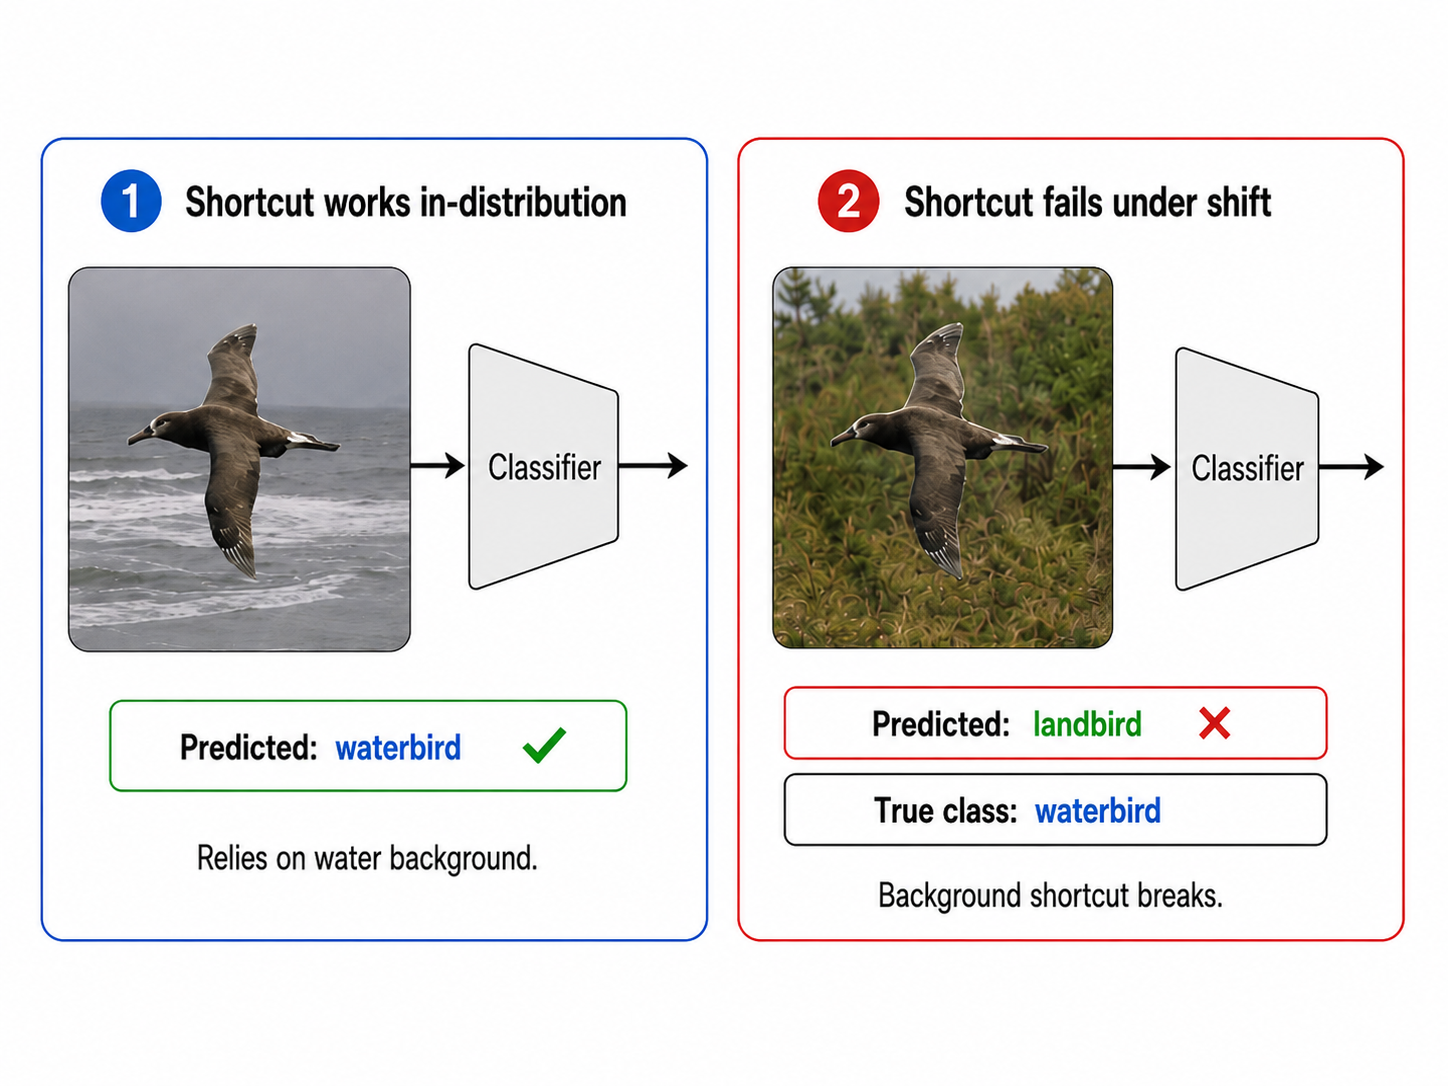
\includegraphics[width=0.95\linewidth]{figs/intro.png}
    \vspace{-3mm}
    \caption{\textbf{Shortcut learning under distribution shift.} When training data spuriously correlates class labels with background, a classifier may learn to use context rather than object evidence}
    \label{fig:intro}
\end{figure}

Vision--language models (VLMs)~\cite{lin2023clip} offer a scalable alternative source of spatial supervision. Because VLMs connect visual regions with natural-language concepts, they can provide weak localization cues from task-level prompts without requiring per-image human masks~\cite{elhoseiny2013write, frome2013devise, lampert2013attribute, le2020using, radford2021learning}. Recent work like GALS~\cite{petryk2022guiding} uses language-grounded spatial maps to guide classifier training, through input-gradient regularization. However, in shortcut-learning settings, gradient suppression is primarily a negative constraint: \textit{it tells the model where not to rely}. It does not directly specify where class evidence should be allocated. Moreover, input-gradient explanations can be noisy, and optimizing classification and explanation constraints jointly from the beginning can be unstable when shortcut features are highly predictive early in training.

In this work, we propose \textbf{Right for the Right Regions (R4RR)}, a training framework that converts VLM-derived localization into a positive, latent evidence-alignment signal for robust classification. Instead of penalizing input gradients on distracting pixels, R4RR aligns the student's spatial class evidence with a soft semantic localization map produced by a frozen VLM teacher~\cite{zhang2025frozen}. Concretely, the teacher provides a nonnegative task-relevant localization map from language prompts, while the student produces a spatial evidence map for the ground-truth class. We normalize both maps into spatial probability distributions and minimize a teacher-to-student KL divergence. This encourages the model to allocate class evidence to semantically relevant regions while preserving uncertainty in the teacher map, avoiding brittle hard masks.

A key component of R4RR is its \emph{Classify-then-Align} training schedule. We first train a model with cross-entropy to learn discriminative structure, then introduce evidence alignment and optimize the combined objective. Our curriculum ablations show that this schedule is substantially more effective than joint training from scratch or alignment-first training, especially in fully biased settings. We instantiate R4RR with CAM-style evidence maps from the final convolutional features for CNNs ~\cite{zhou2016learning}. Additionally, we show our framework also applies for Vision Transformers, where we construct a patch-space evidence map from transformer attention and patch-token activations, then apply the same distributional KL alignment objective.

%Early in training, CAMs or patch-level evidence maps can be noisy and poorly class-discriminative, making direct alignment unstable. R4RR therefore first learns a basic classifier using cross-entropy, then introduces the VLM-guided evidence alignment objective to redirect class evidence toward task-relevant regions. Our curriculum ablations show that this schedule is substantially more effective than joint training from scratch or alignment-first training, especially in fully biased settings.



We evaluate R4RR on three complementary benchmarks of shortcut learning and distribution shift: \emph{DecoyMNIST}~\cite{erion2021improving}, \emph{Waterbirds} \cite{sagawa2019distributionally}, and \emph{RedMeat}, derived from Food-101~\cite{bossard2014food}. Across all three datasets, \textbf{R4RR} consistently outperforms language-guided attention baseline, \emph{GALS}~\cite{petryk2022guiding}, attention-module baseline, \emph{ABN}~\cite{fukui2019attention}, robust-training baseline, \emph{AFR}~\cite{qiu2023simple}, representation-regularization baseline, \emph{ElRep}~\cite{wen2025elastic}, and standard empirical risk minimization (ERM) baselines. The gains are especially pronounced when training data provides little or no counter-bias evidence, as in the fully biased Waterbirds setting. We further show through Pointing Game~\cite{zhang2018top} that R4RR shifts model evidence toward task-relevant object regions.

Our contributions are:
\begin{enumerate}
\item We introduce \textbf{R4RR}, a VLM-guided training framework that improves shortcut robustness by aligning student spatial evidence with soft semantic localization maps from a frozen vision--language teacher.
\item We propose a positive latent evidence-alignment objective based on teacher-to-student KL divergence over spatial distributions, avoiding the limitations of hard masks and input-gradient suppression.
\item We introduce a practical \emph{Classify-then-Align} schedule and show that it substantially improves robustness over joint or alignment-first training.
\item We demonstrate that R4RR is architecture-general: it applies to ResNet, MobileNet, LeNet, and ViT students through architecture-specific spatial evidence maps.
\item We provide empirical evidence on DecoyMNIST, Waterbirds, and RedMeat showing improved worst-group robustness and better localization of task-relevant evidence.
\end{enumerate}

\section{Related Work}
\label{sec:related}

Right for the Right Reasons (RRR)~\cite{ross2017right} penalizes input gradients on features annotated as irrelevant, while CDEP~\cite{rieger2020interpretations} extends this idea using contextual-decomposition-based feature and interaction attributions. Other explanation-guided approaches use saliency, attention, or concept-level supervision to steer models toward interpretable evidence, including concept-sensitive objectives and human-in-the-loop correction mechanisms~\cite{gupta2023concept,gao2022aligning,schramowski2020making}. These methods require pixel-level masks, bounding boxes, curated concepts, or expert rationales creating a supervision bottleneck.

Earlier vision-and-language and zero-shot recognition methods condition classifiers on attributes or textual descriptions~\cite{elhoseiny2013write,frome2013devise,lampert2013attribute,radford2021learning}, while recent CLIP-based localization and weakly supervised segmentation methods show that language prompts can produce meaningful spatial cues~\cite{lin2023clip,zhang2024frozen}. The most closely related line of work uses these spatial cues to guide classifier attention. GALS~\cite{petryk2022guiding} grounds language specifications with a pretrained VLM and applies an auxiliary explanation regularization loss similar to  Right for the Right Reasons (RRR)~\cite{ross2017right}, discouraging reliance on distracting regions. PARIC~\cite{nautiyal2025paric} is a recent preprint that extends this direction by introducing probabilistic VLM embeddings. %: it samples from probabilistic image/text embeddings, generates multiple CLIP Grad-CAM maps, and aggregates them into a reference attention map for language-guided classification. PARIC focuses on uncertainty-aware attention-map generation and prediction stability, whereas our work focuses on how the spatial prior is used during student training for shortcut robustness.


Attention Branch Network (ABN)~\cite{fukui2019attention} augments a CNN with an attention branch whose output is used both for visualization and classification. Automatic Feature Reweighting (AFR)~\cite{qiu2023simple} improves group robustness by retraining the final layer of an ERM model with weights derived from the model's own errors, without requiring group labels. Elastic Representation (ElRep)~\cite{wen2025elastic} instead regularizes the learned representation to mitigate spurious correlations and improve group robustness. These approaches are complementary to R4RR.


% \paragraph{Architecture-specific and architecture-agnostic spatial evidence.}
% Most explanation-guided objectives are tied to a particular form of explanation, such as input gradients, saliency maps, or CNN attention maps. R4RR is instead formulated around a generic student spatial evidence map. For CNNs such as ResNet and MobileNet, this evidence can be instantiated using CAM-style maps from the final convolutional features~\cite{zhou2016learning}. For Vision Transformers, the same objective can be applied to patch-space evidence maps derived from transformer attention and patch-token activations. This makes R4RR an architecture-agnostic evidence-alignment framework: the teacher map, normalization, KL objective, and Classify-then-Align schedule remain unchanged, while only the student evidence-map construction depends on the architecture.

% \paragraph{From negative suppression to positive evidence allocation.}
% R4RR differs from prior language-guided attention regularization in its training mechanism. GALS and related RRR-style objectives primarily impose a negative constraint: they suppress gradients or attention on regions specified as distracting. In contrast, R4RR treats the VLM map as a soft spatial distribution over task-relevant regions and aligns the student's latent class evidence to this distribution using a teacher-to-student KL divergence. This provides a positive evidence-allocation signal, encouraging the model to place class evidence on semantic foreground regions rather than only penalizing evidence in the background. Our component ablations further separate map quality from training mechanism: replacing GALS maps with stronger VLM maps alone is insufficient, while applying the R4RR objective and schedule to alternative map sources recovers much of the robustness gain.

\section{Methodology}
\label{sec:method}

\subsection{Problem Setup}
Let $\mathcal{D}={(x_i,y_i)}_{i=1}^{N}$ denote a labeled image dataset, where $x_i\in\mathbb{R}^{H\times W\times 3}$ and $y_i\in{1,\ldots,C}$. We consider classification settings where task-irrelevant image regions, such as background, texture, border artifacts, or co-occurring context, are spuriously correlated with the label. A classifier trained only with empirical risk minimization may therefore achieve high training or average test accuracy while relying on these shortcut regions.

We train a student classifier $f_\theta$ that outputs logits $z_\theta(x)\in\mathbb{R}^{C}$ and predicted probabilities $p_\theta(x)=\mathrm{softmax}(z_\theta(x))$. Our goal is to learn a classifier that remains accurate while allocating its spatial evidence to task-relevant regions. We assume access to task-level language descriptions, but not to per-image human masks.

\subsection{Overview}
\label{sec:overview}

Our framework, \textbf{Right for the Right Regions (R4RR)}, uses a frozen vision--language teacher to provide soft spatial localization targets during training. For each training image $x_i$ and label $y_i$, R4RR constructs two maps:
\begin{itemize}
\item a \textbf{teacher localization map} $A^{\mathrm{VLM}}(x_i,y_i)$, produced by a frozen VLM-based localization pipeline from task-level language prompts;
\item a \textbf{student evidence map} $A^{\mathrm{stu}}_\theta(x_i,y_i)$, extracted from the student classifier and indicating where the student places evidence for class $y_i$.
\end{itemize}

R4RR aligns these maps by converting both to spatial probability distributions and minimizing a teacher-to-student KL divergence. This converts the VLM localization prior into a positive evidence-allocation signal: instead of only suppressing evidence in distracting regions (common in RRR-style regularization~\cite{ross2017right}), the student is encouraged to place class evidence on task-relevant regions.

The framework is architecture-agnostic. The teacher map, normalization, KL objective, and training schedule remain unchanged across students. Only the construction of $A^{\mathrm{stu}}_\theta$ depends on the student architecture. For CNNs such as ResNet~\cite{he2016deep} and MobileNetV2~\cite{sandler2018mobilenetv2}, we use CAM-style evidence maps. For ViT-B/16 students~\cite{dosovitskiy2020image}, we use an LGM-ViT-style~\cite{ben2024localization} patch-space evidence map.

\subsection{Teacher: Soft Semantic Localization Maps}
\label{sec:teacher}

For each dataset, we define a set of foreground terms $\mathcal{C}$ corresponding to task-relevant concepts and a set of background or context terms $\mathcal{B}$ corresponding to common distracting regions. These terms are inserted into natural-language prompt templates and encoded by a frozen vision--language model. Prompt details are provided in the supplementary pdf.

Our default teacher follows the WeCLIP+~\cite{zhang2024frozen} pipeline, using OpenAI CLIP with DINO refinement. Given an image $x$ and task-level foreground/background prompts, the teacher first obtains class-conditioned localization seeds using Grad-CAM~\cite{selvaraju2017grad} on the frozen CLIP visual backbone with respect to the text prototypes. These seeds are then refined using WeCLIP+'s refinement module (RFM+), which fuses CLIP and DINO~\cite{caron2021emerging} patch features and leverages CLIP attention to propagate and complete the CAM, producing a nonnegative soft localization map:
\begin{equation}
A^{\mathrm{VLM}}(x,y)\in\mathbb{R}^{H_{\mathrm{img}}\times W_{\mathrm{img}}}_{\ge 0}
\end{equation}

The teacher is used only during training. We precompute and cache teacher maps for the training split and freeze the teacher before student training. At inference time, only the student classifier is used. For our final evaluations, we additionally regenerate maps across seeded runs as a stricter robustness check, verifying that the gains are not tied to a single teacher-map instantiation. The total cached map storage is modest across all datasets; details are reported in the supplementary pdf.


\paragraph{Teacher map preprocessing.}
The teacher map is resized to the spatial resolution of the student evidence map using nearest-neighbor interpolation. Let the student evidence grid have resolution $H_s\times W_s$:
\begin{equation}
A^{\mathrm{VLM}}_{\downarrow}(x,y)
=
\mathrm{Downsample}_{\mathrm{NN}}\big(A^{\mathrm{VLM}}(x,y)\big)
\in
\mathbb{R}^{H_{\mathrm{s}}\times W_{\mathrm{s}}}_{\ge 0}.
\end{equation}

We then normalize the resized map into a spatial probability distribution:
\begin{equation}
\hat{A}^{\mathrm{VLM}}(x,y)[u,v]
=
\frac{A^{\mathrm{VLM}}_{\downarrow}(x,y)[u,v]}{\sum_{u',v'} A^{\mathrm{VLM}}_{\downarrow}(x,y)[u',v']+\epsilon}.
\end{equation}
This soft normalization avoids converting teacher maps into brittle hard masks and preserves uncertainty in the VLM localization prior.

\subsection{Student Spatial Evidence Maps}
\label{sec:student_maps}
R4RR requires a spatial evidence map from the student classifier for the ground-truth class, and the construction of this map depends on the student architecture. For CAM-compatible CNNs, we compute student evidence maps using Class Activation Mapping (CAM)~\cite{zhou2016learning} at the spatial resolution of the final convolutional block. We use standard CAM for ResNet-50~\cite{he2016deep} and MobileNetV2~\cite{sandler2018mobilenetv2}, both of which expose final convolutional features followed by global pooling and a linear classifier. For DecoyMNIST~\cite{erion2021improving}, we use Grad-CAM~\cite{selvaraju2017grad} on the second convolutional layer to match the LeNet-style architecture and prior protocol~\cite{rieger2020interpretations}. We discuss Vision Transformer-specific student evidence in Section~\ref{sec:ViTstudent}.


Let $F_\theta(x)\in\mathbb{R}^{D\times H_{\mathrm{s}}\times W_{\mathrm{s}}}$ denote the last convolutional feature tensor and let $\mathbf{W}\in\mathbb{R}^{C\times D}$ be the linear classifier weights (for $C$ classes). For an image $x$ and class $c$, the (pre-nonlinearity) CAM is
\begin{equation}
\begin{aligned}
\tilde{A}^{\mathrm{cam}}_\theta(x,c)[u,v]
&=
\sum_{d=1}^{D} \mathbf{W}_{c,d}\,F_\theta(x)[d,u,v],\\
&\quad (u,v)\in\{1,\dots,H_{\mathrm{s}}\}\times\{1,\dots,W_{\mathrm{s}}\}.
\end{aligned}
\end{equation}

We use the ground-truth class $c=y$ during training. To obtain a nonnegative spatial map, we apply ReLU followed by per-image min--max normalization.
% \begin{equation}
% A^{\mathrm{stu}}*\theta(x,y)[u,v]=
% \frac{
% R_\theta(x,y)[u,v]-\min_{u',v'}R_\theta(x,y)[u',v']
% }{
% \max_{u',v'}R_\theta(x,y)[u',v']-\min_{u',v'}R_\theta(x,y)[u',v']+\epsilon
% }.
% \end{equation}

After obtaining the student evidence map, we convert it into a spatial probability distribution. We first flatten the $H_s\times W_s$ map and apply a spatial softmax:
\begin{align}
\log \hat{A}^{\mathrm{stu}}_\theta(x,c)[u,v]
=
A^{\mathrm{stu}}_\theta(x,c)[u,v]
- \\ 
\log\!\sum_{u',v'} \exp\!\big(A^{\mathrm{stu}}_\theta(x,c)[u',v']\big).
\end{align}

\subsection{Training Objective}
\label{sec:objective}

The classification loss is standard cross-entropy:
\begin{equation}
\mathcal{L}_{\mathrm{CE}}(\theta)=-\frac{1}{B}
\sum_{i=1}^{B}
\log p_\theta(y_i\mid x_i).
\end{equation}

We align the student distribution to the teacher distribution using KL divergence in the teacher-to-student direction:
\begin{equation}
\mathcal{L}_{\mathrm{align}}(\theta)=\frac{1}{B}
\sum_{i=1}^{B}
\mathrm{KL}\left(
\hat{A}^{\mathrm{VLM}}(x_i,y_i)
\Vert
\hat{A}^{\mathrm{stu}}_\theta(x_i,y_i)
\right),
\end{equation}
where
\begin{equation}
\mathrm{KL}(P\Vert Q)=\sum_{u,v}P[u,v]\log\frac{P[u,v]}{Q[u,v]+\epsilon}.
\end{equation}

Unlike hard masking, the alignment loss does not force binary foreground/background decisions, and unlike input-gradient suppression, it directly specifies where class evidence should be allocated.


The final R4RR objective is
\begin{equation}
\mathcal{L}(\theta)=\mathcal{L}_{\mathrm{CE}}(\theta)
+
\lambda \mathcal{L}_{\mathrm{align}}(\theta),
\label{eq:r4rr_objective}
\end{equation}
where $\lambda>0$ controls the strength of evidence alignment.

\subsection{Classify-then-Align Curriculum}
\label{sec:classify_then_align}

Optimizing Eq.~\eqref{eq:r4rr_objective} from the beginning can be unstable because early student evidence maps are often noisy and poorly class-discriminative. R4RR therefore uses a two-phase \emph{Classify-then-Align} schedule.

\paragraph{Phase 1: classification warmup.}
We first train the student using only cross-entropy until the \emph{attention epoch} $E_{\mathrm{cls}}$:
\begin{equation}
\min_{\theta}\mathcal{L}_{\mathrm{CE}}(\theta).
\end{equation}

We treat $E_{\mathrm{cls}}$ (the epoch at which we activate evidence alignment) as a tunable hyperparameter selected on the validation set. This phase is not intended to eliminate shortcut reliance by itself. Its purpose is to produce minimally meaningful class evidence maps that can later be aligned with the VLM teacher.

\paragraph{Phase 2: evidence alignment.}
After the epoch $E_{\mathrm{cls}}$, we introduce the alignment objective and optimize
\begin{equation}
\min_{\theta}
\mathcal{L}_{\mathrm{CE}}(\theta)
+
\lambda \mathcal{L}_{\mathrm{align}}(\theta).
\end{equation}
This phase redirects the student's class evidence toward the teacher-localized task-relevant regions.

\textbf{Model selection.} We select checkpoints using validation performance after the alignment phase begins. This ensures that the selected model reflects the effect of evidence alignment rather than only the cross-entropy warmup. %Algorithm \ref{alg:r4rr} shows our approach. 


% \begin{algorithm}[t]
% \caption{R4RR Training with VLM-guided Evidence Alignment (Classify-then-Align)}
% \label{alg:r4rr}
% \begin{algorithmic}[1]
% \REQUIRE Dataset $\mathcal{D}$, teacher $\mathrm{VLM}$, prompts $\{\mathcal{T}_c\}_{c=1}^C$, alignment weight $\lambda$, attention epochs $E_{\mathrm{cls}}$, joint epochs $E_{\mathrm{joint}}$
% \STATE \textbf{Precompute teacher maps:} for each $(x_i,y_i)\in\mathcal{D}$ compute $A^{\mathrm{VLM}}(x_i,y_i)$ using $\mathrm{VLM}$ and prompts; store maps.
% \STATE Initialize CNN $f_\theta$.
% \STATE \textbf{Phase 1 (classification):} optimize $\mathcal{L}_{\mathrm{CE}}$ for $E_{\mathrm{cls}}$ epochs.
% \STATE Reset optimizer and scheduler; set the Phase~2 learning rate to $\eta_{\mathrm{joint}} = m \cdot \eta_{\mathrm{base}}$, where the multiplier $m$ is tuned.
% \STATE \textbf{Phase 2 (joint):} optimize $\mathcal{L}_{\mathrm{CE}}+\lambda\mathcal{L}_{\mathrm{align}}$ for $E_{\mathrm{joint}}$ epochs:
% \FOR{epoch $=1$ to $E_{\mathrm{joint}}$}
%     \FOR{minibatch $\{(x_i,y_i)\}_{i=1}^B$}
%         \STATE Compute logits $z_\theta(x_i)$ and $\mathcal{L}_{\mathrm{CE}}$.
%         \STATE Compute CAMs $A^{\mathrm{stu}}_\theta(x_i,y_i)$ and normalize to $\hat{A}^{\mathrm{stu}}_\theta$.
%         \STATE Downsample teacher maps $A^{\mathrm{VLM}}(x_i,y_i)$ to resolution of CAM $H_{\mathrm{s}}\times W_{\mathrm{s}}$ and normalize to $\hat{A}^{\mathrm{VLM}}(x_i,y_i)$.
%         \STATE Compute $\mathcal{L}_{\mathrm{align}}$.
%         \STATE Update $\theta$ using $\mathcal{L}=\mathcal{L}_{\mathrm{CE}}+\lambda\mathcal{L}_{\mathrm{align}}$.
%     \ENDFOR
% \ENDFOR
% \STATE \textbf{Inference:} use $f_\theta$ only (no teacher required).
% \end{algorithmic}
% \end{algorithm}

\section{Experiments}
\label{sec:experiment}

%We evaluate R4RR along three axes. First, we test whether evidence alignment improves robustness to spurious correlations on standard biased classification benchmarks. Second, we evaluate whether the learned evidence maps are better localized on task-relevant regions. Third, we test whether R4RR generalizes by applying the same framework to lightweight CNN and Vision Transformer students.

\subsection{Setup}
\label{sec:setup}

\textbf{Datasets.}
We evaluate our framework on three complementary benchmarks of shortcut learning: \textbf{DecoyMNIST}~\cite{erion2021improving},
\textbf{Waterbirds}~\cite{sagawa2019distributionally} and 
\textbf{RedMeat}~\cite{petryk2022guiding}. For Waterbirds, we evaluate two settings: Waterbirds$_{95}$ where a small fraction of training samples counter the dominant background-label correlation, and Waterbirds$_{100}$ where the label and background are perfectly correlated during training, making this setting challenging. Full dataset details and group/class counts are provided in the supplementary pdf.

\begin{figure*}[h]
\centering
\begin{tikzpicture}
\begin{groupplot}[
    group style={
        group size=2 by 2,
        horizontal sep=1.4cm,
        vertical sep=1.9cm
    },
    width=0.48\textwidth,
    height=0.31\textwidth,
    ybar,
    bar width=3.2pt,
    ymin=0,
    ymax=100,
    ylabel={Accuracy (\%)},
    symbolic x coords={Vanilla,CLIP-Z,CLIP-LR,ElRep,Upweight,ABN,GALS,AFR,R4RR},
    xtick=data,
    xticklabel style={rotate=45, anchor=east, font=\scriptsize},
    yticklabel style={font=\scriptsize},
    label style={font=\scriptsize},
    title style={font=\small},
    legend style={
        font=\scriptsize,
        at={(0.5,1.20)},
        anchor=south,
        legend columns=2,
        /tikz/every even column/.append style={column sep=0.3cm}
    },
    enlarge x limits=0.08,
    grid=major,
    grid style={dotted}
]

% ---------------- DecoyMNIST ----------------
\nextgroupplot[
    title={DecoyMNIST},
    legend to name=mainresultslegend
]
\addplot + [
    bar width = 8.5pt,
] coordinates {
    (Vanilla,45.9)
    (CLIP-Z,55.2)
    (CLIP-LR,88.3)
    (ElRep, 49.9)
    (Upweight,49.2)
    (ABN,80.8)
    (GALS,73.2)
    (AFR,44.6)
    (R4RR,96.6)
};
\addplot + [
    bar width = 8.5pt,
] coordinates {
    (Vanilla,0.0)
    (CLIP-Z,0.0)
    (CLIP-LR,76.2)
    (ElRep, 0.1)
    (Upweight,0.0)
    (ABN,25.2)
    (GALS,26.9)
    (AFR,0.0)
    (R4RR,95.8)
};
\legend{Mean group, Worst group}

% ---------------- Waterbirds-95 ----------------
\nextgroupplot[
    title={Waterbirds$_{95}$}
]
\addplot + [
    bar width = 8.5pt,
]coordinates {
    (Vanilla,87.1)
    (CLIP-Z,73.7)
    (CLIP-LR,80.4)
    (ElRep, 88.7)
    (Upweight,86.7)
    (ABN,84.5)
    (GALS,89.1)
    (AFR,91.9)
    (R4RR,90.2)
};
\addplot + [
    bar width = 8.5pt,
]coordinates {
    (Vanilla,71.2)
    (CLIP-Z,44.1)
    (CLIP-LR,56.2)
    (ElRep, 75.4)
    (Upweight,70.8)
    (ABN,62.9)
    (GALS,76.0)
    (AFR,90.4)
    (R4RR,87.1)
};

% ---------------- Waterbirds-100 ----------------
\nextgroupplot[
    title={Waterbirds$_{100}$}
]
\addplot + [
    bar width = 8.5pt,
]coordinates {
    (Vanilla,70.2)
    (CLIP-Z,73.4)
    (CLIP-LR,63.7)
    (ElRep, 74.0)
    (Upweight,70.9)
    (ABN,69.1)
    (GALS,79.9)
    (AFR,69.6)
    (R4RR,89.1)
};
\addplot + [
    bar width = 8.5pt,
]coordinates {
    (Vanilla,40.3)
    (CLIP-Z,43.8)
    (CLIP-LR,24.6)
    (ElRep, 39.8)
    (Upweight,32.9)
    (ABN,34.6)
    (GALS,57.2)
    (AFR,38.4)
    (R4RR,84.8)
};

% ---------------- RedMeat ----------------
\nextgroupplot[
    title={RedMeat}
]
\addplot + [
    bar width = 8.5pt,
]coordinates {
    (Vanilla,67.3)
    (CLIP-Z,61.5)
    (CLIP-LR,76.6)
    (ElRep, 68.1)
    (Upweight,68.3)
    (ABN,65.6)
    (GALS,71.9)
    (AFR,60.7)
    (R4RR,73.2)
};
\addplot + [
    bar width = 8.5pt,
]coordinates {
    (Vanilla,48.0)
    (CLIP-Z,5.6)
    (CLIP-LR,54.0)
    (ElRep, 49.0)
    (Upweight,47.9)
    (ABN,55.3)
    (GALS,57.0)
    (AFR,58.2)
    (R4RR,60.9)
};

\end{groupplot}
\end{tikzpicture}

\vspace{-0.3em}
\ref{mainresultslegend}

\vspace{-0.5em}
\caption{
\textbf{Main robustness results across datasets.}
We compare standard ERM (\textbf{Vanilla}), class-balanced training (\textbf{Upweight}), zero-shot CLIP (\textbf{CLIP-Z}), linear probing on CLIP features (\textbf{CLIP-LR}), ElRep, ABN, GALS, AFR, and our method (\textbf{R4RR}).
Each panel reports mean group accuracy and worst-group accuracy, averaged over five seeds where applicable. Higher is better.
Exact values and standard deviations are provided in the supplementary material.
}
\label{fig:main_results}
\end{figure*}





\textbf{Baselines.} \textbf{Vanilla} trains the student using standard cross-entropy. \textbf{Upweight}~\cite{petryk2022guiding} uses class-balanced cross-entropy with weights inversely proportional to class frequency. \textbf{CLIP-${Zero}$} and \textbf{CLIP-${LR}$} use OpenAI CLIP RN50~\cite{radford2021learning}. CLIP-${Zero}$ evaluates the frozen model with zero-shot text prompts for the target classes, while CLIP-${LR}$ trains a linear classifier on frozen CLIP image features. Direct zero-shot results for all teacher VLM variants are provided in the supplementary material. \textbf{GALS}~\cite{petryk2022guiding} uses language-grounded maps to guide a classifier through explanation regularization. For GALS, we report the strongest validation-selected variant across tuned CLIP backbones and attention-supervision mechanisms. \textbf{ABN}~\cite{fukui2019attention} augments a CNN with an attention branch trained jointly with the classifier. \textbf{AFR}~\cite{qiu2023simple} starts from an ERM-trained model and retrains the final layer with an automatically weighted loss that emphasizes samples the ERM model predicts poorly. \textbf{ElRep}~\cite{wen2025elastic} adds nuclear- and Frobenius-norm penalties to the learned representation to reduce spurious feature reliance.




\textbf{Metrics.} Following group-robustness evaluation~\cite{sagawa2019distributionally}, we report two group-level metrics: (i) \emph{average group accuracy} (\textbf{Mean$_{Group}$}), which assigns equal weight to each group regardless of frequency, and (ii) \emph{worst-group accuracy}, defined as the minimum accuracy over the four groups (\textbf{Worst$_{Group}$}). Worst-group accuracy is particularly informative because it reflects performance on the minority and bias-conflicting groups (e.g. \emph{waterbird-on-land} in Waterbirds dataset), which degrade most severely when the model relies on spurious background cues. For Waterbirds, groups correspond to the four combinations of bird type and background. For DecoyMNIST, groups correspond to digit classes. For RedMeat, groups correspond to the five target classes. 

\textbf{Student details.} Our main experiments use the same student architectures as prior work for each benchmark. For Waterbirds and RedMeat, we train an ImageNet-pretrained ResNet-50~\cite{he2016deep}. For DecoyMNIST, we train a LeNet-style CNN~\cite{lecun1998gradient}. To test architecture generality, we additionally evaluate R4RR with MobileNetV2~\cite{sandler2018mobilenetv2} and ViT-B/16 students in Section \ref{sec:archgeneralize}. We provide exact training details in the supplementary pdf. 
%R4RR uses a two-phase training schedule. In the first phase, the student is trained with cross-entropy only. In the second phase, we optimize cross-entropy plus the VLM-guided evidence-alignment loss. The teacher maps are precomputed and cached before student training, and the teacher is not used during inference.



\textbf{Hyperparameters and evaluation.}
For each dataset and method, we select hyperparameters using automated validation-based tuning unless otherwise noted. 
For the main ResNet/LeNet experiments and baseline comparisons, we run 50 Optuna~\cite{akiba2019optuna} trials per \emph{(dataset, method)} configuration and choose the best trial by validation performance. 
For the architecture-transfer experiments with MobileNetV2 and ViT-B/16 students, we use a smaller 25-trial Optuna budget per configuration.
Unless otherwise noted, all classification results are reported as mean$\pm$standard deviation over five random seeds.
We provide full hyperparameter optimization details in the supplementary material and release the validation-selected hyperparameters for all methods, variants, and ablations in the accompanying code.

\subsection{Results}\label{sec:results}

Figure~\ref{fig:main_results} shows the comparison between different methods. Due to page constraints, we provide qualitative examples in the supplementary pdf. 

\textbf{DecoyMNIST.} Standard ERM (\textbf{Vanilla}) and class reweighting (\textbf{Upweight}) collapse completely on the bias-conflicting groups, indicating near-total reliance on the decoy cue. Zero-shot CLIP (\textbf{CLIP$-{Z}$}) shows the same failure mode on worst-group accuracy despite improved average performance. In contrast, our method \textbf{(R4RR)} achieves the highest per-group and worst-group accuracy, substantially outperforming all baselines we compare against. 

% \begin{table}[h]
% \caption{DecoyMNIST performance evaluation with test accuracy (mean$\pm$std over 5 runs) comparing standard ERM trained model (\textbf{Vanilla}), class-balanced (\textbf{Upweight}), zero-shot CLIP classifier (\textbf{\textbf{CLIP$_{Zero}$}}), linear probe on CLIP features (\textbf{\textbf{CLIP$_{LR}$}}), \textbf{GALS}~\cite{petryk2022guiding}, \textbf{ABN}~\cite{fukui2019attention}, \textbf{AFR}~\cite{qiu2023simple}, and our proposed method (\textbf{Ours}). Higher is better.}
% \label{tab:decoymnist}
% \resizebox{0.5\textwidth}{!}{%
% \begin{tabular}{@{}lcccccccc@{}}
% \toprule
%  &
%   \textbf{Vanilla} &
%  \textbf{CLIP$_{Zero}$} &
%  \textbf{CLIP$_{LR}$} &
%   \textbf{Upweight} &
%   \textbf{ABN} &
%   \textbf{GALS} &
%   \textbf{AFR} &
%   \textbf{Ours} \\ \midrule
% \textbf{Per$_{Group}$} &
%   45.9\scriptsize$\pm$2.7 &
%   55.2\scriptsize$\pm$0.0 &
%   88.3\scriptsize$\pm$0.0 &
%   49.2\scriptsize$\pm$3.2 &
%   80.8\scriptsize$\pm$6.0 &
%   73.2\scriptsize$\pm$11.3 &
%   44.6\scriptsize$\pm$3.2 &
%   \textbf{96.6\scriptsize$\pm$0.1} \\
% \textbf{Worst$_{Group}$} &
%   0.00\scriptsize$\pm$0.0 &
%   0.00\scriptsize$\pm$0.0 &
%   76.2\scriptsize$\pm$0.0 &
%   0.0\scriptsize$\pm$0.0 &
%   25.2\scriptsize$\pm$17.0 &
%   26.9\scriptsize$\pm$22.8 &
%   0.0\scriptsize$\pm$0.0 &
%   \textbf{95.8\scriptsize$\pm$1.3} \\ \bottomrule
% \end{tabular}%
% }
% \end{table}

\textbf{Waterbirds.}
On Waterbirds$_{95}$, where a small fraction of counter-bias examples is available, AFR performs strongly and R4RR remains competitive while substantially improving over ERM.
The gap is largest on Waterbirds$_{100}$, where background and label are perfectly correlated during training.
In this setting, ERM, class balancing, ABN, AFR, ElRep, and direct VLM classifiers all remain vulnerable to the background shortcut, while R4RR achieves the strongest mean-group and worst-group accuracy.
This suggests that when the training distribution provides no evidence that the shortcut is unreliable, the VLM-derived spatial prior supplies a useful corrective signal, redirecting the student toward bird evidence rather than background evidence.


\textbf{RedMeat.} R4RR improves worst-group accuracy over ERM, class balancing, GALS, ABN, AFR, ElRep, and direct VLM classifiers. CLIP$_{LR}$ obtains the highest mean group accuracy, indicating that frozen CLIP features are strong for average classification on this dataset. However, R4RR obtains the best worst-group accuracy, suggesting that explicitly training the classifier to allocate evidence to the target food region improves robustness on the most difficult classes. 


\subsection{Does R4RR improve localization?}\label{sec:pointing}

Beyond classification performance, we assess whether our training procedure improves \emph{where} the model attends, i.e., whether its explanations concentrate on task-relevant evidence. We use the \emph{Pointing Game} \cite{zhang2018top}, a standard protocol for evaluating spatial explanations. For each input image $x_i$, the Pointing Game requires (i) an explanation map $a_i \in \mathbb{R}^{H\times W}$ produced by the model, and (ii) a binary mask $Z_i \in \{0,1\}^{H\times W}$ indicating task-relevant pixels. A sample is counted as a \emph{hit} if the location of the maximum explanation value lies inside the mask. The Pointing Game score is the average hit rate over the evaluation set. Intuitively, a higher score indicates that the model's peak evidence aligns with the relevant region, suggesting that the model is ``right for the right regions'' rather than relying on spurious context. We use the bird segmentation masks in Waterbirds-95\% and Waterbirds-100\% to define $Z_i$. We report Pointing Game on the validation-selected seed for each method. Figure~\ref{fig:pointing_game} shows that R4RR achieves the highest Pointing Game score in both Waterbirds settings. 


\begin{figure}[t]
\centering
\begin{tikzpicture}
\begin{groupplot}[
    group style={
        group size=2 by 1,
        horizontal sep=1.2cm
    },
    width=0.55\columnwidth,
    height=0.54\columnwidth,
    ybar,
    bar width=5pt,
    ymin=0,
    ymax=100,
    ylabel={Hit rate (\%)},
    symbolic x coords={Vanilla,CLIP-Z,CLIP-LR,ElRep,Upweight,ABN,GALS,AFR,R4RR},
    xtick=data,
    xticklabel style={rotate=60, anchor=east, font=\scriptsize},
    yticklabel style={font=\scriptsize},
    label style={font=\scriptsize},
    title style={font=\small},
    enlarge x limits=0.08,
    grid=major,
    grid style={dotted}
]

% -------- Waterbirds-95 --------
\nextgroupplot[
    title={Waterbirds$_{95}$}
]
\addplot + [
    bar width = 7.5pt,
] coordinates {
    (Vanilla,59.9)
    (CLIP-Z,32.4)
    (CLIP-LR,53.5)
    (ElRep,66.0)
    (Upweight,67.4)
    (ABN,7.8)
    (GALS,69.4)
    (AFR,63.9)
    (R4RR,76.6)
};

% -------- Waterbirds-100 --------
\nextgroupplot[
    title={Waterbirds$_{100}$}
]
\addplot + [
    bar width = 7.5pt,
] coordinates {
    (Vanilla,46.5)
    (CLIP-Z,32.0)
    (CLIP-LR,36.4)
    (ElRep,61.1)
    (Upweight,59.3)
    (ABN,6.5)
    (GALS,59.3)
    (AFR,61.6)
    (R4RR,74.7)
};

\end{groupplot}
\end{tikzpicture}

\vspace{-0.5em}
\caption{
\textbf{Pointing Game evaluation on Waterbirds.}
Hit rate (\%) measures whether the peak activation of the explanation map falls inside the ground-truth bird segmentation mask. Higher is better.
%R4RR achieves the best localization performance on both Waterbirds$_{95}$ and Waterbirds$_{100}$, indicating that evidence alignment improves not only robustness but also spatial grounding on task-relevant object regions.
}
\label{fig:pointing_game}
\end{figure}



\subsection{Architecture Generalization}
\label{sec:archgeneralize}

%The main experiments use LeNet~\cite{lecun1998gradient} and ResNet-50~\cite{he2016deep}. We therefore evaluate R4RR on two additional student families: MobileNet~\cite{howard2017mobilenets}, representing lightweight CNNs, and ViT-B/16, representing transformer-based image classifiers.

\subsubsection{MobileNetV2}






We test architecture transfer by replacing the ResNet-50 student with an ImageNet-pretrained MobileNetV2~\cite{sandler2018mobilenetv2}. R4RR keeps the same teacher maps, KL alignment loss, Classify$\rightarrow$Align schedule, training length, and checkpoint-selection rule. We make MobileNetV2 CAM-compatible by using its final convolutional feature map with a dropout-free GAP+linear head, allowing the same class-specific CAM evidence construction used for ResNet-50. Figure~\ref{fig:mobilenet_transfer} shows that R4RR also improves MobileNetV2 robustness over vanilla training, with the largest gains appearing in worst-group accuracy.

\begin{figure}[t]
\centering
\begin{tikzpicture}
\begin{groupplot}[
    group style={
        group size=3 by 1,
        horizontal sep=0.08cm
    },
    scale only axis,
    width=0.30\columnwidth,
    height=0.32\columnwidth,
    ybar,
    bar width=5.5pt,
    ymin=25,
    ymax=95,
    symbolic x coords={ERM,R4RR},
    xtick=data,
    xticklabel style={font=\scriptsize},
    yticklabel style={font=\scriptsize},
    label style={font=\scriptsize},
    title style={font=\small},
    enlarge x limits=0.55,
    grid=major,
    grid style={dotted},
    error bars/y dir=both,
    error bars/y explicit,
    legend style={
        font=\scriptsize,
        at={(1.58,1.20)},
        anchor=south,
        legend columns=2
    }
]

\nextgroupplot[
    title={Waterbirds$_{95}$},
    ylabel={Accuracy (\%)},
    legend to name=mobilenettransferlegend
]
\addplot coordinates {
    (ERM,81.2) +- (0,0.4)
    (R4RR,86.6) +- (0,0.7)
};
\addplot coordinates {
    (ERM,55.3) +- (0,1.9)
    (R4RR,66.3) +- (0,1.8)
};
\legend{Mean group, Worst group}

\nextgroupplot[
    title={Waterbirds$_{100}$},
    yticklabels=\empty,
    ylabel={}
]
\addplot coordinates {
    (ERM,70.9) +- (0,1.3)
    (R4RR,80.4) +- (0,1.1)
};
\addplot coordinates {
    (ERM,35.0) +- (0,7.0)
    (R4RR,53.8) +- (0,4.3)
};

\nextgroupplot[
    title={RedMeat},
    yticklabels=\empty,
    ylabel={}
]
\addplot coordinates {
    (ERM,67.2) +- (0,0.5)
    (R4RR,71.4) +- (0,0.8)
};
\addplot coordinates {
    (ERM,47.0) +- (0,2.5)
    (R4RR,52.8) +- (0,3.3)
};

\end{groupplot}
\end{tikzpicture}

\vspace{0.10em}
\ref{mobilenettransferlegend}

\vspace{-0.55em}

\caption{
\textbf{MobileNetV2 architecture transfer.}
With a MobileNetV2 student, R4RR still improves over ERM while using CAM-based evidence maps.
}
\label{fig:mobilenet_transfer}
\end{figure}

\subsubsection{Vision Transformer}\label{sec:ViTstudent}

For ViT-B/16 students~\cite{dosovitskiy2020image}, CNN-style CAM is not directly available because the model operates on patch tokens rather than convolutional feature maps. We therefore use a ViT-native patch-space evidence map adapted from the embedding-attention fused explanation map of LGM-ViT~\cite{ben2024localization}. This changes only the student evidence extractor: the VLM teacher maps, teacher-to-student KL loss, and Classify$\rightarrow$Align schedule are unchanged.

Let the final transformer block contain $M$ attention heads and $P=H_sW_s$ patch tokens. We extract two patch-level signals. First, from the final-layer attention tensor $\mathcal{A}^{L}\in\mathbb{R}^{M\times(P+1)\times(P+1)}$, where token $0$ is the CLS token, we compute the averaged CLS-to-patch attention
\begin{equation}
a_p(x)=\frac{1}{M}\sum_{m=1}^{M}\mathcal{A}^{L}_{m,0,p}.
\end{equation}
Second, from the final patch tokens $h_p\in\mathbb{R}^{D}$, we compute an embedding-activation score
\begin{equation}
b_p(x)=\frac{1}{D}\sum_{d=1}^{D}h_{p,d}.
\end{equation}
The ViT evidence score is their weighted fusion,
\begin{equation}
s_p(x)=\beta a_p(x)+(1-\beta)b_p(x),
\end{equation}
with $\beta=0.85$ in our experiments. We reshape $\{s_p\}_{p=1}^{P}$ into an $H_s\times W_s$ patch grid and use it as $A^{\mathrm{stu}}_\theta(x)$ in the same spatial KL alignment objective as the CNN students.


Figure~\ref{fig:vit_transfer} shows that R4RR transfers beyond CNN students: replacing CAMs with a transformer-native patch evidence map still improves ViT robustness across all datasets. The gains are largest on Waterbirds$_{100}$, where no counter-bias examples are available during training, suggesting that the VLM-derived spatial prior remains useful even when evidence is represented over patch tokens rather than convolutional feature maps. These results support R4RR as an architecture-general evidence-alignment framework rather than a CAM-specific CNN regularizer.


\begin{figure}[t]
\centering
\begin{tikzpicture}
\begin{groupplot}[
    group style={
        group size=3 by 1,
        horizontal sep=0.08cm
    },
    scale only axis,
    width=0.30\columnwidth,
    height=0.32\columnwidth,
    ybar,
    bar width=5.5pt,
    ymin=25,
    ymax=95,
    symbolic x coords={ERM,R4RR},
    xtick=data,
    xticklabel style={font=\scriptsize},
    yticklabel style={font=\scriptsize},
    label style={font=\scriptsize},
    title style={font=\small},
    enlarge x limits=0.55,
    grid=major,
    grid style={dotted},
    error bars/y dir=both,
    error bars/y explicit,
    legend style={
        font=\scriptsize,
        at={(1.58,1.20)},
        anchor=south,
        legend columns=2
    }
]

\nextgroupplot[
    title={Waterbirds$_{95}$},
    ylabel={Accuracy (\%)},
    legend to name=vittransferlegend
]
\addplot coordinates {
    (ERM,79.4) +- (0,0.7)
    (R4RR,86.1) +- (0,1.2)
};
\addplot coordinates {
    (ERM,55.9) +- (0,3.0)
    (R4RR,72.1) +- (0,4.5)
};
\legend{Mean group, Worst group}

\nextgroupplot[
    title={Waterbirds$_{100}$},
    yticklabels=\empty,
    ylabel={}
]
\addplot coordinates {
    (ERM,69.6) +- (0,0.6)
    (R4RR,83.2) +- (0,0.5)
};
\addplot coordinates {
    (ERM,36.8) +- (0,2.4)
    (R4RR,61.8) +- (0,2.6)
};

\nextgroupplot[
    title={RedMeat},
    yticklabels=\empty,
    ylabel={}
]
\addplot coordinates {
    (ERM,68.1) +- (0,0.4)
    (R4RR,73.1) +- (0,0.5)
};
\addplot coordinates {
    (ERM,49.4) +- (0,3.2)
    (R4RR,56.8) +- (0,2.4)
};

\end{groupplot}
\end{tikzpicture}

\vspace{0.1em}
\ref{vittransferlegend}

\vspace{-0.55em}
\caption{
\textbf{R4RR transfers to ViT-B/16 students.}
Using an EAFEM-style patch-space evidence map, R4RR improves over ViT ERM.
}
\label{fig:vit_transfer}
\end{figure}




\section{Ablation studies}\label{sec:ablation}

\subsection{Study on teacher selection}
\begin{figure}[t]
\centering
\begin{tikzpicture}
\begin{groupplot}[
    group style={
        group size=1 by 2,
        vertical sep=1.85cm
    },
    width=0.93\columnwidth,
    height=0.43\columnwidth,
    ybar,
    bar width=5pt,
    ymin=75,
    ymax=93,
    ylabel={Accuracy (\%)},
    symbolic x coords={CLIP+DINO,OCLIP+DINO,SigLIP2+DINO,CLIP+XCiT},
    xtick=data,
    xticklabel style={rotate=25, anchor=east, font=\scriptsize},
    yticklabel style={font=\scriptsize},
    label style={font=\scriptsize},
    title style={font=\small},
    legend style={
        font=\scriptsize,
        at={(0.5,1.22)},
        anchor=south,
        legend columns=2
    },
    enlarge x limits=0.13,
    grid=major,
    grid style={dotted},
    error bars/y dir=both,
    error bars/y explicit
]
% ---------------- Waterbirds-95 ----------------
\nextgroupplot[
    title={Waterbirds$_{95}$},
    legend to name=teacherlegend
]
\addplot+[error bars/.cd, y dir=both, y explicit] coordinates {
    (CLIP+DINO,90.2) +- (0,0.7)
    (OCLIP+DINO,90.5) +- (0,0.3)
    (SigLIP2+DINO,90.3) +- (0,0.3)
    (CLIP+XCiT,90.4) +- (0,0.3)
};
\addplot+[error bars/.cd, y dir=both, y explicit] coordinates {
    (CLIP+DINO,87.1) +- (0,2.7)
    (OCLIP+DINO,88.1) +- (0,0.9)
    (SigLIP2+DINO,87.4) +- (0,0.9)
    (CLIP+XCiT,88.0) +- (0,1.2)
};
\legend{Mean group, Worst group}

% ---------------- Waterbirds-100 ----------------
\nextgroupplot[
    title={Waterbirds$_{100}$}
]
\addplot+[error bars/.cd, y dir=both, y explicit] coordinates {
    (CLIP+DINO,89.1) +- (0,0.4)
    (OCLIP+DINO,89.1) +- (0,0.5)
    (SigLIP2+DINO,88.0) +- (0,0.8)
    (CLIP+XCiT,89.1) +- (0,0.3)
};
\addplot+[error bars/.cd, y dir=both, y explicit] coordinates {
    (CLIP+DINO,84.8) +- (0,1.0)
    (OCLIP+DINO,85.6) +- (0,1.8)
    (SigLIP2+DINO,81.6) +- (0,0.8)
    (CLIP+XCiT,84.0) +- (0,1.3)
};

\end{groupplot}
\end{tikzpicture}
\vspace{-0.4em}
\ref{teacherlegend}
\vspace{-0.15em}
\caption{
\textbf{Teacher ablation on Waterbirds.}
We vary the VLM backbone and refinement backbone while keeping the student, loss, and training curriculum fixed.
\textbf{OCLIP+DINO} denotes OpenCLIP with DINO refinement, and \textbf{CLIP+XCiT} denotes CLIP with XCiT-DINO refinement.
%R4RR is relatively stable across teacher choices; OpenCLIP+DINO is slightly strongest on worst-group accuracy, while SigLIP2+DINO drops more in the fully biased Waterbirds$_{100}$ setting.
}
\label{fig:teacher_ablation}
\end{figure}



Our default teacher follows WeCLIP+~\cite{zhang2024frozen}, which combines CLIP and DINO. Here, we test the sensitivity of \textbf{R4RR} to the teacher by swapping (i) the VLM backbone (CLIP $\rightarrow$ OpenCLIP~\cite{openclip} with LAION-pretrained weights or SigLIP2~\cite{siglip2}) and (ii) the refinement backbone (DINO $\rightarrow$ XCiT-DINO~\cite{el2021xcit, caron2021emerging}), while keeping the student, prompts, loss, and curriculum fixed.

Figure~\ref{fig:teacher_ablation} shows that \textbf{R4RR} is largely insensitive to the teacher choice: all variants maintain strong Mean$_{Group}$ accuracy in both bias settings. OpenCLIP is consistently best (or tied) on Worst$_{Group}$, while SigLIP2 drops on Waterbirds$_{100}$, suggesting that teacher calibration matters most when training is fully biased. This trend carries over to other datasets, discussed in the supplementary pdf.

\subsection{Sensitivity to hyperparameters and teacher-map quality}
\label{sec:sensitivity_stress}


We further test whether \textbf{R4RR} depends on a fragile operating point or perfectly accurate teacher maps. First, we perform a local sensitivity study on Waterbirds$_{100}$ by perturbing one \textbf{R4RR}-specific hyperparameter at a time around the validation-selected configuration: the alignment start epoch, the KL alignment weight, and the Phase-2 learning-rate multiplier. 
Across these perturbations, performance remains stable: mean group accuracy stays within $88.4$--$89.1$, and worst-group accuracy stays within $82.5$--$85.1$, compared to $89.1\pm0.4$ mean group and $84.8\pm1.0$ worst-group accuracy for the tuned configuration. Full sensitivity details are provided in the supplementary pdf. 

Second, we stress-test \textbf{R4RR} under imperfect teacher supervision by corrupting a fixed 15\% subset of training teacher maps before student training. We consider two corruption types: aggressive Gaussian blur, which makes the teacher map spatially diffuse, and inversion, which creates an actively misleading teacher signal. \textbf{R4RR} remains stable across all datasets, with the largest worst-group drop occurring on RedMeat, the noisiest benchmark, while Waterbirds and DecoyMNIST show little to no degradation. These results indicate that \textbf{R4RR} benefits from the overall structure of teacher-guided evidence alignment rather than relying on a razor-thin hyperparameter setting or perfectly accurate teacher maps for every training example. Full corruption details are provided in the supplementary pdf.

\subsection{Teacher maps vs.\ objective/schedule}
\label{sec:ablation_gals_vs_r4rr}
To disentangle why \textbf{R4RR} improves over GALS~\cite{petryk2022guiding} which also uses VLM-guided maps, we factor the gain into (i) the \emph{training mechanism} (our KL evidence-alignment with a two-phase warm-start) and (ii) the \emph{teacher map construction} (WeCLIP+~\cite{zhang2024frozen}). We compare: (A) \emph{GALS objective + our teacher maps}, (B) \emph{R4RR objective/schedule + GALS RN50 maps}, (C) \emph{R4RR objective/schedule + GALS maps}, (D) \emph{R4RR (ours)}: R4RR objective/schedule + teacher maps.

\begin{figure}[t]
\centering
\begin{tikzpicture}
\begin{groupplot}[
    group style={
        group size=1 by 3,
        vertical sep=1.1cm
    },
    width=0.93\columnwidth,
    height=0.34\columnwidth,
    ybar,
    bar width=6pt,
    ymin=40,
    ymax=95,
    ylabel={Accuracy (\%)},
    symbolic x coords={A,B,C,D},
    xtick=data,
    xticklabels={A,B,C,D},
    xticklabel style={font=\scriptsize},
    yticklabel style={font=\scriptsize},
    label style={font=\scriptsize},
    title style={font=\small},
    legend style={
        font=\scriptsize,
        at={(0.5,1.22)},
        anchor=south,
        legend columns=2
    },
    enlarge x limits=0.18,
    grid=major,
    grid style={dotted},
    error bars/y dir=both,
    error bars/y explicit
]

% ---------------- Waterbirds-95 ----------------
\nextgroupplot[
    title={Waterbirds$_{95}$},
    legend to name=galsr4rrlegend
]
\addplot+[error bars/.cd, y dir=both, y explicit] coordinates {
    (A,87.0) +- (0,0.4)
    (B,89.4) +- (0,0.3)
    (C,86.1) +- (0,1.5)
    (D,90.2) +- (0,0.7)
};
\addplot+[error bars/.cd, y dir=both, y explicit] coordinates {
    (A,70.4) +- (0,2.6)
    (B,83.8) +- (0,1.5)
    (C,71.6) +- (0,4.7)
    (D,87.1) +- (0,2.7)
};
\legend{Mean group, Worst group}

% ---------------- Waterbirds-100 ----------------
\nextgroupplot[
    title={Waterbirds$_{100}$}
]
\addplot+[error bars/.cd, y dir=both, y explicit] coordinates {
    (A,73.2) +- (0,2.2)
    (B,87.7) +- (0,0.3)
    (C,85.4) +- (0,0.1)
    (D,89.1) +- (0,0.5)
};
\addplot+[error bars/.cd, y dir=both, y explicit] coordinates {
    (A,40.9) +- (0,9.4)
    (B,76.2) +- (0,1.7)
    (C,72.6) +- (0,2.0)
    (D,85.6) +- (0,1.8)
};

% ---------------- RedMeat ----------------
\nextgroupplot[
    title={RedMeat}
]
\addplot+[error bars/.cd, y dir=both, y explicit] coordinates {
    (A,71.8) +- (0,0.7)
    (B,68.9) +- (0,1.5)
    (C,67.4) +- (0,1.1)
    (D,73.2) +- (0,1.0)
};
\addplot+[error bars/.cd, y dir=both, y explicit] coordinates {
    (A,57.4) +- (0,2.2)
    (B,52.3) +- (0,6.2)
    (C,51.0) +- (0,2.4)
    (D,60.9) +- (0,3.4)
};

\end{groupplot}
\end{tikzpicture}

\vspace{0.1em}
\ref{galsr4rrlegend}

\vspace{-0.5em}
\caption{
\textbf{GALS vs.\ R4RR component ablation.}
We separate the effects of the teacher-map source and the training objective/schedule.
\textbf{(A)} GALS objective + our teacher maps.
\textbf{(B)} R4RR objective/schedule + GALS RN50 maps.
\textbf{(C)} R4RR objective/schedule + GALS ViT maps.
\textbf{(D)} Full R4RR: R4RR objective/schedule + our teacher maps.
%Across datasets, replacing the training mechanism yields a larger gain than replacing the teacher maps alone, and the full combination performs best overall.
}
\label{fig:gals_r4rr_ablation}
\end{figure}


Figure~\ref{fig:gals_r4rr_ablation} shows that map quality alone is not sufficient: \textbf{GALS + our maps (A)} remains brittle under full bias (Waterbirds$_{100}$ worst-group $40.9$). In contrast, swapping \emph{only} the training mechanism (\textbf{R4RR objective + GALS maps (B--C)}) recovers most of the robustness on Waterbirds, indicating that aligning {latent} evidence under a warm-started two-phase schedule is the primary driver. Finally, \textbf{R4RR} with WeCLIP+ maps performs best across datasets, suggesting the two components are complementary: our schedule provides the main robustness gain, while segmentation-style pseudo-masks further strengthen the alignment target, especially in the fully biased and noisy settings.


\subsection{Training curriculum}
\label{sec:ablationtrainingcuriculum}

R4RR uses a two-phase \textbf{Classify$\rightarrow$Align} schedule: the student first learns with $\mathcal{L}_{\mathrm{CE}}$, then optimizes $\mathcal{L}_{\mathrm{CE}}+\lambda\mathcal{L}_{\mathrm{align}}$. We compare this schedule with \textbf{Align$\rightarrow$Classify} and \textbf{Joint} training and discover that Classify$\rightarrow$Align is consistently strongest, especially on Waterbirds$_{100}$ worst-group accuracy. This indicates that CE warmup does not remove shortcuts by itself, but provides meaningful class evidence that the alignment phase can redirect toward task-relevant regions. Full results are in the supplementary material.

\section{Limitations}
\textbf{R4RR} precomputes and caches teacher maps for efficiency during student training. While this avoids repeated teacher inference, storing dense maps can be memory-intensive for large datasets or high resolutions. An interesting direction is to generate maps on-the-fly (possibly at lower spatial resolution) to remove the caching requirement. Similarly, although our teacher-selection ablations suggest that \textbf{R4RR} is relatively insensitive to the specific CLIP-family backbone, the approach can still inherit failure modes of the underlying VLM. 


\section{Conclusion}
In this work, we presented \textbf{Right for the Right Regions (R4RR)}, a scalable framework that reduces shortcut reliance by aligning a student’s \emph{latent spatial evidence} with task-relevant regions provided by a frozen vision--language teacher, using a two-phase \emph{Classify-then-Align} training curriculum that warm-starts discriminative learning before introducing evidence alignment. Across three complementary spurious-correlation benchmarks (Waterbirds, DecoyMNIST, and RedMeat), \textbf{R4RR} consistently improves robustness and generalization over standard ERM training and strong baselines spanning language-guided attention supervision, attention-branch architectures, and lightweight reweighting. 


%\textcolor{red}{somewhere in the results:}{We do not claim that cross-entropy warmup prevents shortcut learning by itself. Rather, the warmup makes the student's evidence map sufficiently meaningful for alignment.}
\input{sec/2_formatting}
\input{sec/3_finalcopy}
{
    \small
    \bibliographystyle{ieeenat_fullname}
    \bibliography{main}
}
% \newpage 
% \appendix

% \noindent\textbf{Table of Contents}
% \begin{itemize}
%   \item \ref{appendix:qualisamples} Qualitative samples \dotfill \pageref{appendix:qualisamples}
%   \item \ref{appendix:prompts} Prompts \dotfill \pageref{appendix:prompts}
%    \item \ref{appendix:implementation_details} Implementation Details \dotfill \pageref{appendix:implementation_details}
% \item \ref{appendix:teacher_map_cost} Teacher map storage \dotfill \pageref{appendix:teacher_map_cost}
%     \item \ref{sec:hparam_opt} Hyperparameter Optimization \dotfill \pageref{sec:hparam_opt}
%      \item \ref{appendix:r4rroptimized} R4RR Optimized Hyperparameters \dotfill \pageref{appendix:r4rroptimized}
%      \item \ref{appendix:r4rr_sensitivity} Local sensitivity to R4RR hyperparameters \dotfill \pageref{appendix:r4rr_sensitivity}
%      \item \ref{appendix:teacher_map_corruption} Teacher-map corruption stress test \dotfill \pageref{appendix:teacher_map_corruption}
%       \item \ref{appendix:vlmablation} Teacher ablation on additional datasets \dotfill \pageref{appendix:vlmablation}
%         \item \ref{sec:supp_dataset_splits} Dataset splits \dotfill \pageref{sec:supp_dataset_splits}

%   \item \ref{sec:supp_gals_optuna_variants} Additional GALS Optimization \dotfill \pageref{sec:supp_gals_optuna_variants}
%    % \item \ref{appendix:prompts} Prompts \dotfill \pageref{appendix:prompts}
%    % \item \ref{appendix:prompts} Prompts \dotfill \pageref{appendix:prompts}
% \end{itemize}


% \section{Dataset}
% \subsection{Details}\label{datasetdetails}
% \textbf{DecoyMNIST}~\cite{erion2021improving} is a digit-classification benchmark in which class-indicative gray patches are added to the image boundary. A classifier predicts the digit class from the decoy rather than from the digit itself.

% \textbf{Waterbirds}~\cite{sagawa2019distributionally}  is a benchmark constructed by placing bird images from CUB~\cite{wah2011caltech}  on land or water backgrounds from Places~\cite{zhou2017places}. The target label is bird type, landbird or waterbird, while the background is spuriously correlated with the label during training. We evaluate two settings. In Waterbirds$_{95}$, a small fraction of training samples counter the dominant background-label correlation. In Waterbirds$_{100}$, the label and background are perfectly correlated during training, making this setting especially challenging.

% \textbf{RedMeat}~\cite{petryk2022guiding} is a 5-way classification task derived from Food-101~\cite{bossard2014food}, with classes baby back ribs, filet mignon, pork chop, prime rib, and steak. The training data contains implicit biases and noisy context, including label noise, sauces, plates, side dishes, and other co-occurring visual artifacts. The test split is cleaner, so models that rely on training-only artifacts generalize poorly.
% \section{Splits}
% \label{sec:supp_dataset_splits}

% Tables \ref{tab:splits_decoymnist}, \ref{tab:splits_waterbirds95}, \ref{tab:splits_waterbirds100} and \ref{tab:splits_redmeat} report the train/validation/test splits used in all experiments. For DecoyMNIST, we create the validation set by taking a stratified 10\% slice from the original training split (per digit), and we report the resulting counts below.

% % -------------------- DecoyMNIST --------------------
% \begin{table}[h]
% \centering
% \caption{\textbf{DecoyMNIST class-balanced splits (counts per digit).} Validation is a stratified 10\% slice from the original training split.}
% \label{tab:splits_decoymnist}
% \scriptsize
% \setlength{\tabcolsep}{3pt}
% \renewcommand{\arraystretch}{1.15}
% \resizebox{\linewidth}{!}{%
% \begin{tabular}{l cccccccccc}
% \toprule
% \textbf{Split} & \textbf{0} & \textbf{1} & \textbf{2} & \textbf{3} & \textbf{4} & \textbf{5} & \textbf{6} & \textbf{7} & \textbf{8} & \textbf{9} \\
% \midrule
% Train      & 5331 & 6068 & 5362 & 5518 & 5258 & 4879 & 5326 & 5638 & 5266 & 5354 \\
% Validation &  592 &  674 &  596 &  613 &  584 &  542 &  592 &  627 &  585 &  595 \\
% Test       &  980 & 1135 & 1032 & 1010 &  982 &  892 &  958 & 1028 &  974 & 1009 \\
% \bottomrule
% \end{tabular}%
% }
% \end{table}

% % -------------------- Waterbirds-95 --------------------
% \begin{table}[h]
% \centering
% \caption{\textbf{Waterbirds$_{95}$ splits (group counts).} Groups are the four label$\times$background combinations.}
% \label{tab:splits_waterbirds95}
% \scriptsize
% \setlength{\tabcolsep}{4pt}
% \renewcommand{\arraystretch}{1}
% \begin{tabular}{l cccc}
% \toprule
% \textbf{Split} &
% \textbf{Landbird, Land} &
% \textbf{Landbird, Water} &
% \textbf{Waterbird, Land} &
% \textbf{Waterbird, Water} \\
% \midrule
% Train      & 3498 & 184 &  56 & 1057 \\
% Val &  467 & 466 & 133 &  133 \\
% Test       & 2255 & 2255 & 642 &  642 \\
% \bottomrule
% \end{tabular}
% \end{table}

% % -------------------- Waterbirds-100 --------------------
% \begin{table}[h]
% \centering
% \caption{\textbf{Waterbirds$_{100}$ splits (group counts).} Training is fully biased (no counter-biased groups).}
% \label{tab:splits_waterbirds100}
% \scriptsize
% \setlength{\tabcolsep}{4pt}
% \renewcommand{\arraystretch}{1.15}
% \begin{tabular}{l cccc}
% \toprule
% \textbf{Split} &
% \textbf{Landbird, Land} &
% \textbf{Landbird, Water} &
% \textbf{Waterbird, Land} &
% \textbf{Waterbird, Water} \\
% \midrule
% Train      & 3684 &   0 &   0 & 1111 \\
% Val &  465 & 466 & 134 &  134 \\
% Test       & 2255 & 2255 & 642 &  642 \\
% \bottomrule
% \end{tabular}
% \end{table}

% % -------------------- RedMeat --------------------
% \begin{table}[h]
% \centering
% \caption{\textbf{RedMeat splits (class counts).} Classes follow \cite{petryk2022guiding}.}
% \label{tab:splits_redmeat}
% \scriptsize
% \setlength{\tabcolsep}{4pt}
% \renewcommand{\arraystretch}{1.15}
% \begin{tabular}{l ccccc}
% \toprule
% \textbf{Split} &
% \textbf{Baby Back Ribs} &
% \textbf{Filet Mignon} &
% \textbf{Pork Chop} &
% \textbf{Prime Rib} &
% \textbf{Steak} \\
% \midrule
% Train      & 500 & 500 & 500 & 500 & 500 \\
% Val & 250 & 250 & 250 & 250 & 250 \\
% Test       & 250 & 250 & 250 & 250 & 250 \\
% \bottomrule
% \end{tabular}
% \end{table}






% \section{Qualitative samples}\label{appendix:qualisamples}
% We demonstrate saliency maps for \emph{RedMeat}~\cite{petryk2022guiding}, \emph{DecoyMNIST}~\cite{erion2021improving} and \emph{Waterbirds}~\cite{sagawa2019distributionally} in Figures~\ref{fig:appendixredmeat}, \ref{fig:appendixMNIST}, and \ref{fig:appendixwaterbird}.

% \begin{figure}[h]
%     \centering
%     \includegraphics[width=0.95\linewidth]{figs/redmeat_resized.jpg}
%     \caption{\textbf{Right for the wrong regions vs.\ right for the right regions on RedMeat.} Comparing saliency maps between our method, \emph{GALS}~\cite{petryk2022guiding}, standard \emph{vanilla} model, \emph{ABN}~\cite{fukui2019attention}, \emph{AFR}~\cite{qiu2023simple} and class balanced model (\emph{Upweight}). Shortcut-prone models often attend to spurious context (e.g., background).} 
%      \label{fig:appendixredmeat}
% \end{figure}

% \begin{figure}
%     \centering
%     \includegraphics[width=0.95\linewidth]{figs/decoymnist_resized.jpg}
%     \caption{\textbf{Right for the wrong regions vs.\ right for the right regions on DecoyMNIST.} Comparing saliency maps between our method, \emph{GALS}~\cite{petryk2022guiding}, standard \emph{vanilla} model, \emph{ABN}~\cite{fukui2019attention}, \emph{AFR}~\cite{qiu2023simple} and class balanced model (\emph{Upweight}). Shortcut-prone models often attend to spurious context (e.g., background).} 
%     \label{fig:appendixMNIST}
% \end{figure}


% \begin{figure}
%     \centering
%     \includegraphics[width=0.98\linewidth]{figs/waterbirds100_resized.jpg}
%     \caption{\textbf{Right for the wrong regions vs.\ right for the right regions on Waterbirds.} Comparing saliency maps between our method, \emph{GALS}~\cite{petryk2022guiding}, standard \emph{vanilla} model, \emph{ABN}~\cite{fukui2019attention}, \emph{AFR}~\cite{qiu2023simple} and class balanced model (\emph{Upweight}). Shortcut-prone models often attend to spurious context (e.g., background).} 
%      \label{fig:appendixwaterbird}
% \end{figure}


% % \begin{figure*}[t]
% %     \centering
% %     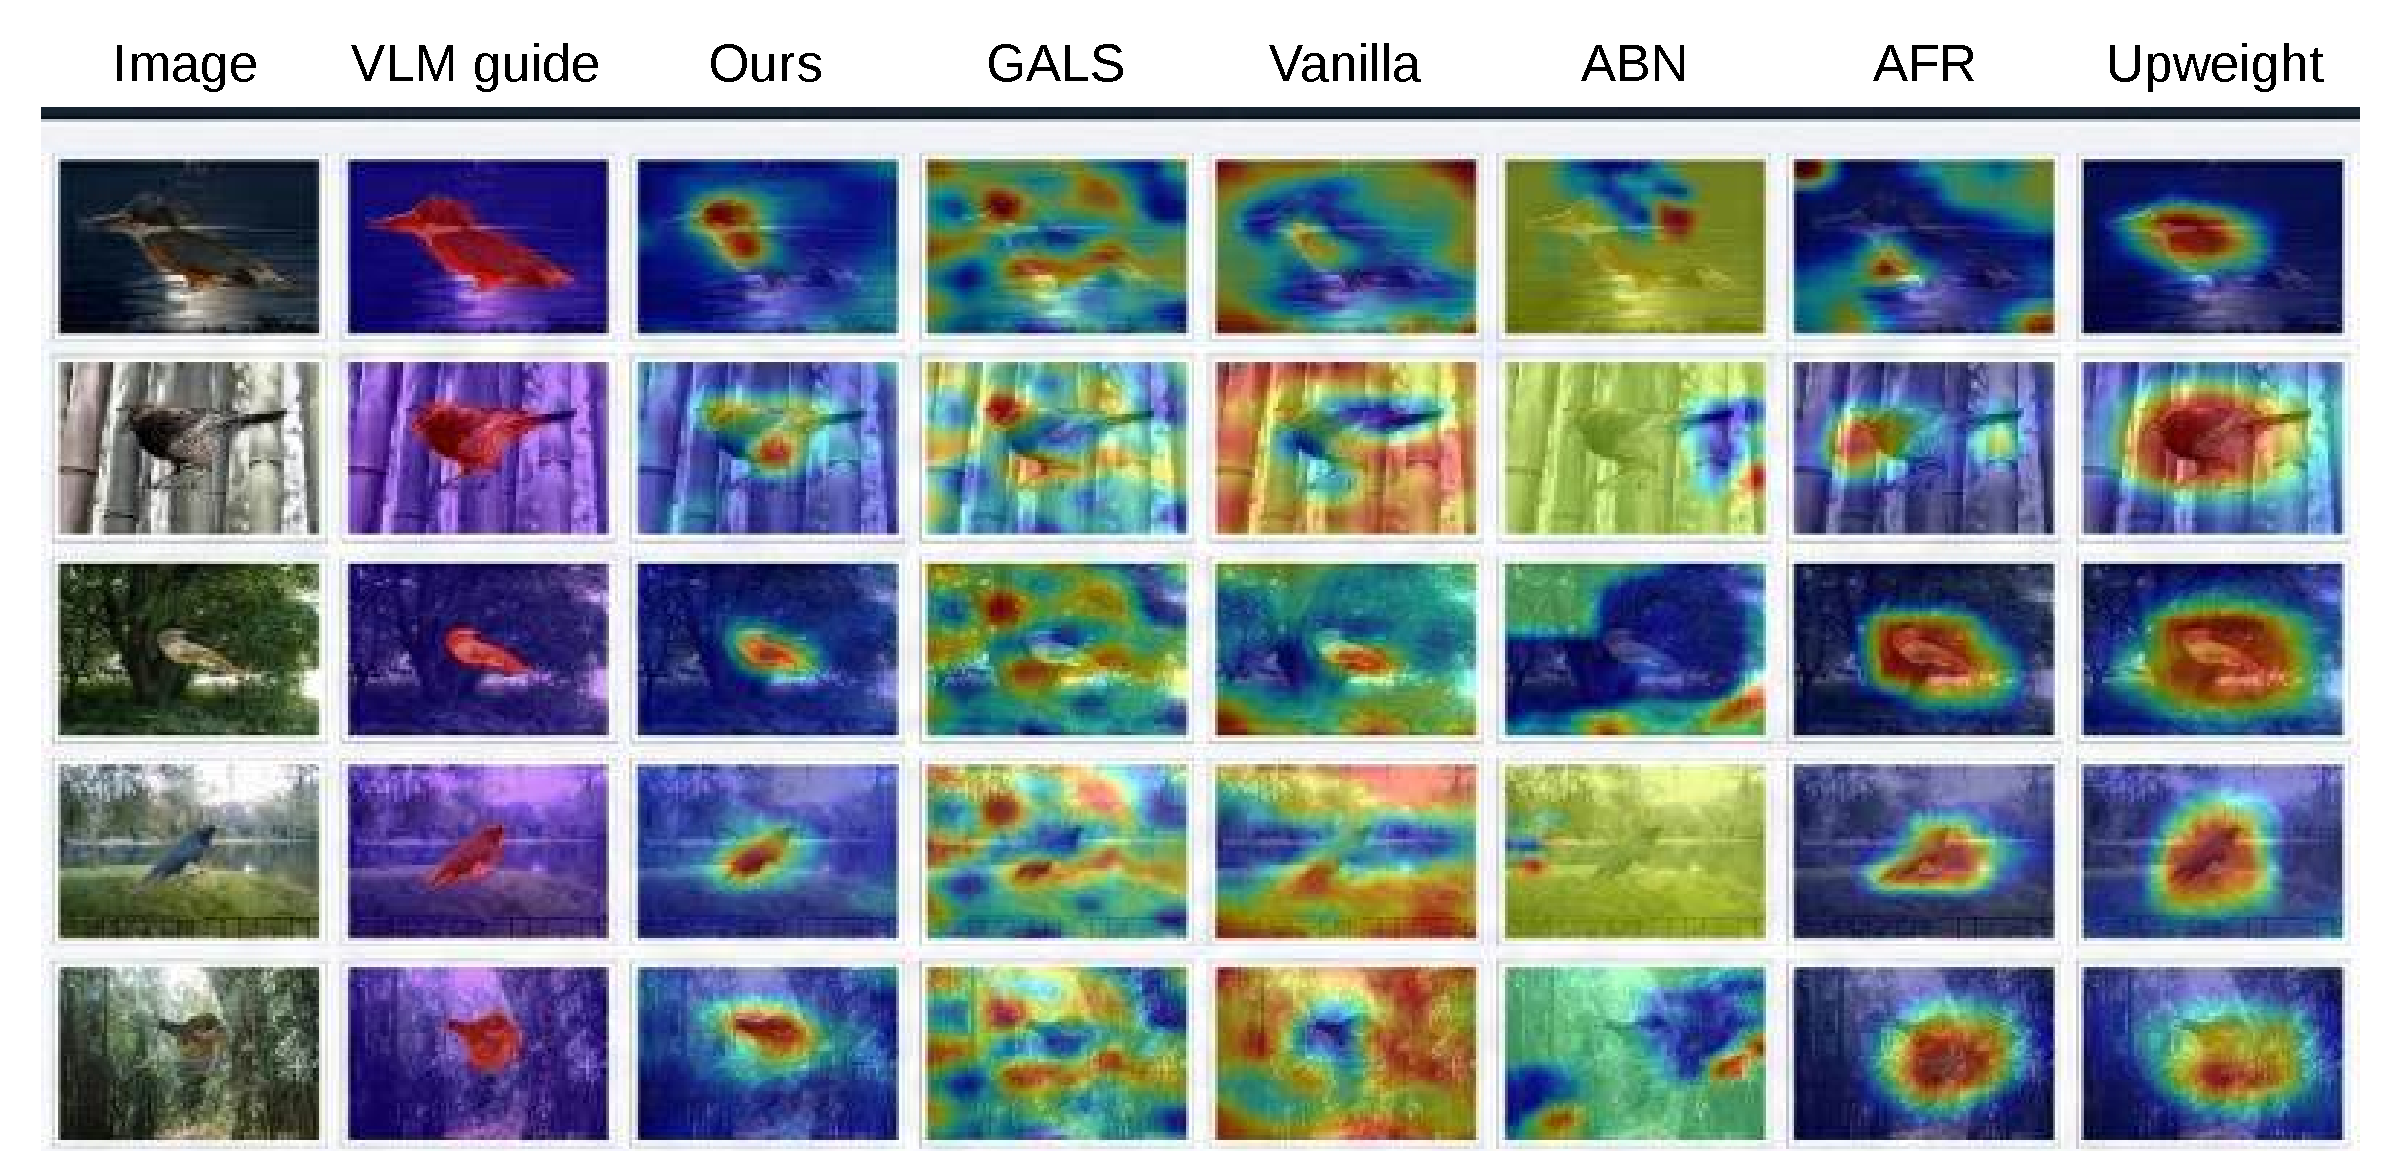
\includegraphics[width=0.98\linewidth]{figs/home.drawio-compressed.pdf}
% %     \caption{\textbf{Right for the wrong regions vs.\ right for the right regions.} Comparing saliency maps between our method, \emph{GALS}~\cite{petryk2022guiding}, standard \emph{vanilla} model, \emph{ABN}~\cite{fukui2019attention}, \emph{AFR}~\cite{qiu2023simple} and class balanced model (\emph{Upweight}). Shortcut-prone models often attend to spurious context (e.g., background).} 
% %     %Our method aligns the student CNN's latent spatial evidence (CAMs) with VLM-derived semantic affinity maps, avoiding shortcut leqrning with spurious features.}
% %     \label{fig:waterbird}
% % \end{figure*}



% \section{Prompts}\label{appendix:prompts}

% Table~\ref{tab:task_level_prompts} shows the task level prompts for each dataset. 

% \begin{table}[h]
% \centering
% \caption{Task-level foreground prompts used to generate VLM teacher maps.}
% \label{tab:task_level_prompts}
% \small
% \setlength{\tabcolsep}{6pt}
% \renewcommand{\arraystretch}{1.05}
% \begin{tabular}{ll}
% \toprule
% \textbf{Dataset} & \textbf{Task-level prompt} \\
% \midrule
% Waterbirds & \texttt{"a clean origami of bird"} \\
% RedMeat    & \texttt{"a clean origami of meat"} \\
% DecoyMNIST & \texttt{"a clean origami of digit"} \\
% \bottomrule
% \end{tabular}
% \end{table}



% \paragraph{Why use the prompt \texttt{``a clean origami of \{t\}.''}?}
% We adopt the fixed prompt wrapper \texttt{``a clean origami of \{t\}.''} because our teacher-map generator follows the same CLIP-based weakly supervised segmentation pipeline used by WeCLIP+~\cite{zhang2024frozen}. In this line of work, prompt wording is part of the pseudo-label generator itself, and prior CLIP-WSSS work reports that prompt choice can materially affect the quality of CLIP Grad-CAM pseudo labels. In particular, the original CLIP-based segmentation method underlying this family found that prompt modifiers such as \texttt{clean} could improve segmentation quality and selected \texttt{``a clean origami of \{\}.''} as its fixed template~\cite{lin2023clip}. We therefore keep that template unchanged when constructing teacher maps, so that our study isolates the effect of \textbf{R4RR}'s evidence-alignment objective and training curriculum rather than introducing an additional prompt-engineering variable.

% We additionally use a set of \emph{background} (distractor) prompts to represent common contextual regions that frequently co-occur with the foreground object and may serve as spurious cues.


% \paragraph{Selecting background prompts.}
% Background prompt selection is lightweight and dataset-driven. For datasets that are predominantly outdoor (e.g., Waterbirds), we include distractors that commonly appear in outdoor scenes (e.g., terrain and natural context). For primarily indoor datasets, we instead include indoor-relevant distractors (e.g., furniture and man-made interiors). We also reuse the general-purpose background terms provided in our repository as a strong default; in practice these general distractors are effective and reduce the need to hand-engineer dataset-specific lists. Background/distractor prompt files are provided in our repository under \texttt{WeCLIPPlus/clip/clip\_texts/}.


% \section{Implementation Details}
% \label{appendix:implementation_details}

% \subsection{Model Details by Dataset}\label{appendix:model_details}
% \paragraph{Waterbirds.}
% \begin{itemize}
%     \item \textbf{Student:} ResNet-50\cite{he2016deep} (ImageNet pretrained), inputs resized to $224\times224$ with ImageNet normalization. 
%     \item \textbf{Training:} SGD (momentum $0.9$, weight decay $10^{-5}$), batch size $96$, $200$ epochs. 
% \end{itemize}

% R4RR uses CAM from the final convolutional block; teacher maps are resized to the CAM grid. Alignment is enabled only after the warm-start phase (attention epoch). Model selection uses validation performance computed after alignment is introduced.

% \paragraph{RedMeat.}
% \begin{itemize}
%     \item \textbf{Student:} ResNet-50\cite{he2016deep} (ImageNet pretrained), $224\times224$ with ImageNet normalization. 
%     \item \textbf{Training:} SGD (momentum $0.9$, weight decay $10^{-5}$), batch size $96$, $150$ epochs. 
% \end{itemize}

% As in Waterbirds, R4RR uses standard CAM from the final convolutional block, with teacher maps resized to the CAM grid. R4RR follows the same Classify$\rightarrow$Joint schedule and validation protocol as Waterbirds.

% \paragraph{DecoyMNIST.}
% \begin{itemize}
%     \item \textbf{Student:} LeNet-style CNN on $28\times28$ grayscale inputs normalized to $[-1,1]$. 
%     \item \textbf{Training:} Adam (weight decay $10^{-4}$), learning rate $10^{-3}$, $19$ epochs (for all methods), model selection by validation accuracy. 
% \end{itemize}
% Evidence maps use Grad-CAM on the second convolutional layer. The $19$-epoch budget matches Waterbirds training exposure: $200\cdot 4750/50000 \approx 19$. R4RR again uses Classify$\rightarrow$Joint, with selection performed after alignment is enabled.







% \subsection{Teacher map storage}
% \label{appendix:teacher_map_cost}

% R4RR uses fixed VLM-derived teacher maps that are generated offline before student training. For hyperparameter optimization, these maps are cached once per dataset and then reused across the full set of Optuna sweeps, so the teacher preprocessing cost is not incurred separately for each hyperparameter trial. In practice, this one-time caching strategy is the natural deployment setting: once the teacher maps are generated, they can be reused throughout tuning and training. For the final five-seed evaluations, however, we regenerate teacher maps separately for each seed and pair them with the corresponding seeded run. This is not required for efficiency, but is a stricter fairness check: it verifies that the reported gains are not tied to a single fixed teacher-map randomization and continue to hold under different seeded instantiations of the teacher preprocessing pipeline.

% The resulting cached teacher maps have a modest storage footprint. Table~\ref{tab:teacher_map_cost} reports the total on-disk size for the full set of generated teacher maps for each dataset, not for a single image. Across all datasets, the cached supervision remains lightweight to store and reuse.

% \begin{table}[h]
% \centering
% \caption{\textbf{Cached teacher-map storage.} Total on-disk size for the full set of generated teacher maps for each dataset.}
% \label{tab:teacher_map_cost}
% \small
% \setlength{\tabcolsep}{8pt}
% \renewcommand{\arraystretch}{1.1}
% \begin{tabular}{lc}
% \toprule
% \textbf{Dataset} & \textbf{Total cached size} \\
% \midrule
% Waterbirds$_{95}$  & 19\,MB \\
% Waterbirds$_{100}$ & 19\,MB \\
% RedMeat            & 12\,MB \\
% DecoyMNIST         & 30\,MB \\
% \bottomrule
% \end{tabular}
% \end{table}





% \subsection{Hyperparameter Optimization}
% \label{sec:hparam_opt}

% Unless stated otherwise, we tune hyperparameters \emph{separately} for each dataset (Waterbirds$_{95}$, Waterbirds$_{100}$, RedMeat) and \emph{separately} for each method and configuration (e.g., each GALS variant is swept independently). For most methods, we run 50 Optuna trials~\cite{akiba2019optuna} per \emph{(dataset, method)} setting and choose the best trial using validation performance. On Waterbirds, we select by group-aware validation accuracy (Per$_{Group}$); on RedMeat, we select by standard validation accuracy for the 5-way task. Reported test numbers are mean$\pm$std over five seeds (0--4). Experiments were run on a university HPC cluster with NVIDIA A100 PCIe 40\,GB GPUs and Intel Xeon Gold 6150 CPUs (2.70\,GHz).


% For GALS~\cite{petryk2022guiding}, we tune both the default configuration and several design variants under the same Optuna budget, including (i) CLIP ViT vs.\ CLIP RN50 as the language-attention source and (ii) different classifier-attention mechanisms (RRR, Grad-CAM, and ABN). Unless otherwise stated, we report the strongest tuned GALS variant per dataset under this common budget.

% See Table \ref{tab:sweep_spaces_summary} and \ref{tab:sweep_spaces_def}. 



% \FloatBarrier
% \begin{table}[!ht]
% \centering
% \caption{Hyperparameter tuning summary. Search spaces S1--S9 are defined in Table~\ref{tab:sweep_spaces_def}. Unless noted, $\texttt{weight\_decay}=10^{-5}$ is fixed by the method configuration. Most deep methods use 50 Optuna trials \cite{akiba2019optuna} per dataset; CLIP-ZS is not tuned.}
% \label{tab:sweep_spaces_summary}
% \scriptsize
% \setlength{\tabcolsep}{3pt}
% \renewcommand{\arraystretch}{1.15}
% \begin{tabularx}{\linewidth}{l l X l}
% \toprule
% \textbf{Family} & \textbf{Variant} & \textbf{Tuned} & \textbf{Space} \\
% \midrule
% \multirow{3}{*}{GALS (RRR-style)}
% & RN50     & \texttt{base\_lr}, \texttt{classifier\_lr}, \texttt{grad\_weight}, \texttt{grad\_criterion} & S1 \\
% & ViT      & \texttt{base\_lr}, \texttt{classifier\_lr}, \texttt{grad\_weight}, \texttt{grad\_criterion} & S1 \\
% & OurMasks & \texttt{base\_lr}, \texttt{classifier\_lr}, \texttt{grad\_weight}, \texttt{grad\_criterion} & S1 \\
% \midrule
% GALS+GradCAM & ViT & \texttt{base\_lr}, \texttt{classifier\_lr}, \texttt{cam\_weight} & S2 \\
% GALS+ABN     & ViT & \texttt{base\_lr}, \texttt{classifier\_lr}, \texttt{abn\_att\_weight} & S3 \\
% Upweight     & --- & \texttt{base\_lr}, \texttt{classifier\_lr} & S4 \\
% ABN baseline & --- & \texttt{base\_lr}, \texttt{classifier\_lr}, \texttt{abn\_cls\_weight} & S5 \\
% Vanilla CNN  & --- & \texttt{base\_lr}, \texttt{classifier\_lr}, \texttt{momentum} & S6 \\
% \midrule
% \multirow{3}{*}{Ours (R4RR)}
% & OurMasks & \texttt{attention\_epoch}, \texttt{kl\_lambda}, \texttt{base\_lr}, \texttt{classifier\_lr}, \texttt{lr2\_mult} & S7 \\
% & RN50     & \texttt{attention\_epoch}, \texttt{kl\_lambda}, \texttt{base\_lr}, \texttt{classifier\_lr}, \texttt{lr2\_mult} & S7 \\
% & ViT      & \texttt{attention\_epoch}, \texttt{kl\_lambda}, \texttt{base\_lr}, \texttt{classifier\_lr}, \texttt{lr2\_mult} & S7 \\
% \midrule
% CLIP+LR & --- & \texttt{C} & S8 \\
% CLIP-ZS & --- & (none; fixed evaluation) & --- \\
% \midrule
% AFR (two-stage grid; not Optuna) & --- & \texttt{gamma}, \texttt{reg\_coeff} & S9 \\
% \bottomrule
% \end{tabularx}
% \end{table}
% \FloatBarrier


% \begin{table}[!ht]
% \centering
% \caption{Search space definitions referenced in Table~\ref{tab:sweep_spaces_summary}. Ranges apply when running Optuna sweeps, unless the method is explicitly noted as a grid (AFR). For \texttt{attention\_epoch}, we sweep over valid epoch indices: $0..199$ for Waterbirds (200 epochs) and $0..149$ for RedMeat (150 epochs).}
% \label{tab:sweep_spaces_def}
% \scriptsize
% \setlength{\tabcolsep}{3pt}
% \renewcommand{\arraystretch}{1.15}
% \begin{tabularx}{\linewidth}{l X}
% \toprule
% \textbf{ID} & \textbf{Definition} \\
% \midrule
% S1 & $\texttt{base\_lr}\in[10^{-5},5\cdot10^{-2}]$ (log), $\texttt{classifier\_lr}\in[10^{-5},5\cdot10^{-2}]$ (log), $\texttt{grad\_weight}\in[10^{3},10^{5}]$ (log), $\texttt{grad\_criterion}\in\{\texttt{L1},\texttt{L2}\}$ \\
% S2 & $\texttt{base\_lr}\in[5\cdot10^{-4},5\cdot10^{-2}]$ (cfg-centered), $\texttt{classifier\_lr}\in[10^{-5},10^{-3}]$ (cfg-centered), $\texttt{cam\_weight}\in[10^{-2},10^{2}]$ (log) \\
% S3 & $\texttt{base\_lr}\in[10^{-3},10^{-1}]$, $\texttt{classifier\_lr}\in[10^{-4},10^{-2}]$, $\texttt{abn\_att\_weight}\in[10^{-2},10^{2}]$ (log) \\
% S4 & $\texttt{base\_lr}\in[5\cdot10^{-5},10^{-1}]$, $\texttt{classifier\_lr}\in[5\cdot10^{-5},10^{-1}]$ \\
% S5 & $\texttt{base\_lr}\in[5\cdot10^{-5},10^{-1}]$, $\texttt{classifier\_lr}\in[5\cdot10^{-5},10^{-1}]$, $\texttt{abn\_cls\_weight}\in[10^{-2},10^{2}]$ (log) \\
% S6 & $\texttt{base\_lr}\in[10^{-5},5\cdot10^{-2}]$ (log), $\texttt{classifier\_lr}\in[10^{-5},5\cdot10^{-2}]$ (log), $\texttt{momentum}\in[0.85,0.95]$ \\
% S7 & $\texttt{attention\_epoch}\in\{0,\dots,E-1\}$ ($E{=}200$ Waterbirds, $E{=}150$ RedMeat), $\texttt{kl\_lambda}\in[1,500]$ (log), $\texttt{base\_lr}\in[10^{-5},5\cdot10^{-2}]$ (log), $\texttt{classifier\_lr}\in[10^{-5},5\cdot10^{-2}]$ (log), $\texttt{lr2\_mult}\in[10^{-1},3]$ (log) \\
% S8 & $\texttt{C}\in[10^{-2},10^{2}]$ (log) \\
% S9 & (AFR grid; not Optuna) full-paper grid: $\texttt{gamma}\in\{4.0,4.5,\dots,20.0\}$ (33 values), $\texttt{reg\_coeff}\in\{0,0.1,0.2,0.3,0.4\}$ (5 values), for $33\times5=165$ stage-2 configurations per seed. Reduced grids are also supported for debugging. \\
% \bottomrule
% \end{tabularx}
% \end{table}
% \FloatBarrier

% \paragraph{AFR tuning protocol.} AFR~\cite{qiu2023simple} follows a two-stage procedure that differs from the Optuna sweeps above. For each dataset and seed, we (i) train a standard ERM backbone once, then (ii) freeze the backbone and retrain only the final layer while exhaustively sweeping a fixed grid over (\texttt{gamma}, \texttt{reg\_coeff}). A ``trial'' corresponds to one (\texttt{gamma}, \texttt{reg\_coeff}) pair for one seed (stage-2 only). We use the full grid with $\texttt{gamma}\in\{4.0,4.5,\dots,20.0\}$ and $\texttt{reg\_coeff}\in\{0,0.1,0.2,0.3,0.4\}$, totaling $165$ stage-2 configurations per seed. Within each seed, we select the grid point that maximizes validation worst-group accuracy (\texttt{best\_val\_wga}) and report the corresponding test performance at that validation-selected point $\newline$ (\texttt{best\_test\_at\_val}); we then aggregate mean$\pm$std over seeds 0--4.



% \paragraph{DecoyMNIST tuning protocol.}
% We do not tune hyperparameters directly on DecoyMNIST because, in our setting, a validation split drawn from the DecoyMNIST training data is not a reliable proxy for the test-time objective. Since the training set remains fully biased, model selection within that same distribution can favor configurations that fit the decoy shortcut rather than those that genuinely improve robustness under shift. Instead, we treat DecoyMNIST as an out-of-distribution stress test and transfer hyperparameters from Waterbirds$_{100}$, motivated by the fact that both correspond to fully biased training regimes. This choice is intended to be conservative rather than opportunistic: we do not perform dataset-specific hyperparameter search for our method on DecoyMNIST, and the resulting performance should therefore be interpreted as transfer from one fully biased benchmark to another rather than as the outcome of DecoyMNIST-specific tuning. To match compute across datasets, we also align the approximate number of training-image exposures rather than epochs. Because DecoyMNIST uses a single global learning rate, we fix it to $10^{-3}$ and set \texttt{attention\_epoch} by exposure matching. For DecoyMNIST, the reported GALS result uses the same transferred GALS variant selected on Waterbirds$_{100}$, namely the CLIP ViT + RRR-style configuration.


% \subsection{R4RR Optimized Hyperparameters}\label{appendix:r4rroptimized}


% \paragraph{Reproducibility (full tuned configs).}
% For full reproducibility, we release the $\newline$
% validation-selected hyperparameters for \textbf{all} methods, variants, and ablations (for each dataset) in our codebase under \texttt{configs/}. This directory contains dataset- and method-specific YAML configuration files corresponding to the runs reported in the main paper and supplementary material.

% \paragraph{Best R4RR hyperparameters.}
% Table~\ref{tab:r4rr_best_hparams} reports the validation-selected R4RR hyperparameters used for our main results. For Waterbirds and RedMeat, we report the single best Optuna trial per dataset. For DecoyMNIST, we do not tune; we reuse the Waterbirds$_{100}$ configuration and set \texttt{attention\_epoch} by matching training-image exposures (19 total epochs $\Rightarrow$ \texttt{attention\_epoch}=7).


% \paragraph{\texttt{lr2\_mult}.}
% We use a two-phase schedule where Phase~2 (joint optimization with evidence alignment) resets the optimizer. \texttt{lr2\_mult} is a multiplicative factor applied to the learning rates at the start of Phase~2, i.e., $\texttt{base\_lr}^{(2)}=\texttt{lr2\_mult}\cdot \texttt{base\_lr}$ and $\texttt{classifier\_lr}^{(2)}=\texttt{lr2\_mult}\cdot \texttt{classifier\_lr}$, allowing Phase~2 to run with a smaller or larger step size than Phase~1.


% \FloatBarrier
% \begin{table}[t]
% \centering
% \caption{\textbf{R4RR best hyperparameters.} Best validation-selected configuration per dataset for our method. Waterbirds uses $E{=}200$ epochs, RedMeat uses $E{=}150$. DecoyMNIST uses $E{=}19$ and does not tune hyperparameters; we use fixed Adam learning rates and set \texttt{attention\_epoch} by exposure-matching to WB$_{100}$.}
% \label{tab:r4rr_best_hparams}
% \scriptsize
% \setlength{\tabcolsep}{4pt}
% \renewcommand{\arraystretch}{0.3}
% \begin{tabular}{lccccc}
% \toprule
% \textbf{Dataset} &
% \texttt{att\_ep} &
% \texttt{kl\_lambda} &
% \texttt{base\_lr} &
% \texttt{classifier\_lr} &
% \texttt{lr2\_mult} \\
% \midrule
% Waterbirds$_{95}$  & 109 & 295.30 & $4.82{\times}10^{-5}$ & $2.93{\times}10^{-3}$ & 0.409 \\
% Waterbirds$_{100}$ & 73  & 495.61 & $5.72{\times}10^{-5}$ & $3.57{\times}10^{-3}$ & 0.123 \\
% DecoyMNIST         & 7   & 495.61 & $1.00{\times}10^{-3}$ & $1.00{\times}10^{-3}$ & 0.123 \\
% RedMeat            & 2   & 11.44  & $2.40{\times}10^{-3}$ & $2.33{\times}10^{-4}$ & 1.567 \\
% \bottomrule
% \end{tabular}
% \end{table}
% \FloatBarrier








% \section{Local sensitivity to R4RR-specific hyperparameters}
% \label{appendix:r4rr_sensitivity}

% To assess whether \textbf{R4RR} depends on a narrowly tuned operating point, we perform a lightweight local sensitivity study around the validation-selected configuration on Waterbirds$_{100}$. Starting from the best hyperparameters reported in Table~\ref{tab:r4rr_best_hparams}, we perturb one R4RR-specific hyperparameter at a time while holding the others fixed. We consider the three method-specific quantities introduced by our two-phase evidence-alignment framework: the alignment start epoch  $\newline$ (\texttt{attention\_epoch}), the evidence-alignment weight (\texttt{kl\_lambda}), and the Phase-2 learning-rate multiplier (\texttt{lr2\_mult}). Each perturbed configuration is evaluated over the same five seeds (0--4) used in the main paper.

% \begin{table}[h]
% \centering
% \caption{\textbf{Local sensitivity of R4RR-specific hyperparameters on Waterbirds$_{100}$.} Starting from the validation-selected R4RR configuration, we perturb one hyperparameter at a time while keeping all others fixed. Results are test accuracy (mean$\pm$std over 5 seeds). Higher is better.}
% \label{tab:r4rr_local_sensitivity}
% \small
% \setlength{\tabcolsep}{8pt}
% \renewcommand{\arraystretch}{1.1}
% \begin{tabular}{lcc}
% \toprule
% \textbf{Setting} & \textbf{Per$_{Group}$} & \textbf{Worst$_{Group}$} \\
% \midrule
% \texttt{attention\_epoch} + 10 & 88.9\scriptsize$\pm$0.5 & 83.1\scriptsize$\pm$2.6 \\
% \texttt{attention\_epoch} - 10 & 89.0\scriptsize$\pm$0.2 & 83.9\scriptsize$\pm$2.5 \\
% \texttt{lr2\_mult} $\times$ 0.75 & 88.8\scriptsize$\pm$0.8 & 83.8\scriptsize$\pm$2.0 \\
% \texttt{lr2\_mult} $\times$ 1.25 & 89.0\scriptsize$\pm$0.3 & 84.9\scriptsize$\pm$1.7 \\
% \texttt{kl\_lambda} $\times$ 0.75 & 88.4\scriptsize$\pm$0.4 & 82.5\scriptsize$\pm$1.5 \\
% \texttt{kl\_lambda} $\times$ 1.25 & 88.8\scriptsize$\pm$0.2 & 85.1\scriptsize$\pm$1.6 \\
% \midrule
% Best tuned config & 89.1\scriptsize$\pm$0.4 & 84.8\scriptsize$\pm$1.0 \\
% \bottomrule
% \end{tabular}
% \end{table}

% Table~\ref{tab:r4rr_local_sensitivity} shows that \textbf{R4RR} remains strong under moderate one-at-a-time perturbations of its main method-specific hyperparameters. Across all tested settings, Per$_{Group}$ varies only within a narrow range ($88.4$--$89.1$), and Worst$_{Group}$ remains similarly stable ($82.5$--$85.1$). In particular, modest shifts in the alignment start epoch and the Phase-2 learning-rate multiplier have only small effects on performance, while changes to \texttt{kl\_lambda} lead to somewhat larger but still limited variation. Importantly, none of these nearby settings causes a collapse in worst-group accuracy, indicating that the gains of \textbf{R4RR} do not rely on an extremely fragile choice of hyperparameters.

% Overall, this local sensitivity study supports the view that \textbf{R4RR} is reasonably robust around its validation-selected operating point: the tuned setting remains among the strongest, but neighboring configurations continue to deliver high group-balanced performance in the fully biased Waterbirds$_{100}$ regime. This is encouraging because it suggests that the benefits of evidence alignment arise from the method itself rather than from a razor-thin hyperparameter choice.





% \section{Teacher-map corruption stress test}
% \label{appendix:teacher_map_corruption}

% Because \textbf{R4RR} relies on precomputed VLM-derived teacher maps, an important question is how sensitive the method is to imperfections in those maps. To study this, we perform a lightweight \emph{teacher-map corruption stress test} in which we deliberately degrade a fixed subset of teacher maps before student training and then train \textbf{R4RR} with all other settings unchanged.

% \paragraph{Setup.}
% For each dataset, we start from the same validation-selected \textbf{R4RR} hyperparameters used in the main paper and supplementary material. We then randomly select a fixed 15\% subset of training examples (using a fixed seed), corrupt the corresponding teacher maps once before training, and keep those same corrupted maps fixed throughout the entire run. This design tests robustness to \emph{persistent} teacher errors rather than transient optimization noise. We consider two corruption types:

% \begin{itemize}
%     \item \textbf{Blur 15\%:} for the selected 15\% of training examples, we apply an \emph{aggressive} Gaussian blur to each teacher map (OpenCV Gaussian blur; kernel \(31\times31\), \(\sigma_x=\sigma_y=10.0\)). We then clamp values to be nonnegative and renormalize each map to sum to 1. If a blurred map is degenerate (near-zero total mass), we replace it with a uniform map before renormalization. This models strongly spatially diffuse, imprecise teacher supervision rather than mild smoothing.
%     \item \textbf{Invert 15\%:} replace the selected teacher maps with their inverted versions ($1-M$, followed by renormalization). This creates an intentionally \emph{wrong} teacher signal that suppresses originally high-response regions and emphasizes irrelevant regions instead.
% \end{itemize}

% All other aspects of training remain unchanged, including the student architecture, curriculum, optimizer settings, and checkpoint-selection protocol. We report mean$\pm$std over the same five seeds used in the main paper.


% \begin{table}[t]
% \centering
% \caption{\textbf{Teacher-map corruption stress test.} Test accuracy (mean$\pm$std over 5 seeds) for \textbf{R4RR} under fixed corruption of 15\% of training teacher maps. \emph{Clean} denotes the standard unmodified teacher maps used in the main paper. \emph{Blur 15\%} applies strong Gaussian blur to a fixed subset of teacher maps, while \emph{Invert 15\%} replaces a fixed subset with inverted maps. Higher is better.}
% \label{tab:teacher_map_corruption}
% \small
% \setlength{\tabcolsep}{6pt}
% \renewcommand{\arraystretch}{1.12}
% \resizebox{0.92\linewidth}{!}{%
% \begin{tabular}{llcc}
% \toprule
% \textbf{Dataset} & \textbf{Teacher-map condition} & \textbf{Per$_{Group}$} & \textbf{Worst$_{Group}$} \\
% \midrule
% \multirow{3}{*}{DecoyMNIST}
% & Clean       & 96.6\scriptsize$\pm$0.1 & 95.8\scriptsize$\pm$1.3 \\
% & Blur 15\%   & 96.7\scriptsize$\pm$0.19 & 95.5\scriptsize$\pm$0.7 \\
% & Invert 15\% & 96.8\scriptsize$\pm$0.2 & 95.6\scriptsize$\pm$0.8 \\
% \midrule
% \multirow{3}{*}{RedMeat}
% & Clean       & 73.2\scriptsize$\pm$1.0 & 60.9\scriptsize$\pm$3.4 \\
% & Blur 15\%   & 72.6\scriptsize$\pm$1.5 & 58.7\scriptsize$\pm$4.6 \\
% & Invert 15\% & 72.8\scriptsize$\pm$1.1 & 59.4\scriptsize$\pm$5.2 \\
% \midrule
% \multirow{3}{*}{Waterbirds$_{100}$}
% & Clean       & 89.1\scriptsize$\pm$0.4 & 84.8\scriptsize$\pm$1.0 \\
% & Blur 15\%   & 88.8\scriptsize$\pm$0.5 & 85.0\scriptsize$\pm$1.4 \\
% & Invert 15\% & 88.7\scriptsize$\pm$0.4 & 84.0\scriptsize$\pm$0.8 \\
% \midrule
% \multirow{3}{*}{Waterbirds$_{95}$}
% & Clean       & 90.2\scriptsize$\pm$0.7 & 87.1\scriptsize$\pm$2.7 \\
% & Blur 15\%   & 90.2\scriptsize$\pm$0.3 & 88.0\scriptsize$\pm$0.9 \\
% & Invert 15\% & 90.1\scriptsize$\pm$0.3 & 87.0\scriptsize$\pm$0.8 \\
% \bottomrule
% \end{tabular}%
% }
% \end{table}

% Table~\ref{tab:teacher_map_corruption} shows that \textbf{R4RR} remains strong under moderate teacher corruption. Across all four dataset settings, corrupting 15\% of the training teacher maps causes only limited changes in performance relative to the clean-teacher reference. On \textbf{DecoyMNIST}, performance is essentially unchanged under both blur and inversion, indicating that \textbf{R4RR} does not require perfectly accurate teacher localization on every example in this highly structured fully biased regime. On \textbf{Waterbirds$_{95}$} and \textbf{Waterbirds$_{100}$}, the results are similarly stable: Per$_{Group}$ remains near the clean baseline, and Worst$_{Group}$ changes only modestly, with no evidence of collapse even when part of the teacher supervision is deliberately corrupted.

% The largest degradation appears on \textbf{RedMeat}, where both corruption types reduce Worst$_{Group}$ accuracy by a small amount relative to the clean setting. This is consistent with RedMeat being the noisiest and least structured benchmark in our suite: when the task itself contains label noise, co-occurring food context, and fine-grained visual ambiguity, imperfect teacher localization is somewhat more harmful. Even so, the corrupted-teacher models remain close to the clean \textbf{R4RR} result, indicating that the method still functions effectively under moderate teacher degradation.

% These results support two conclusions. First, the gains of \textbf{R4RR} do not depend on every teacher map being perfectly precise. A fixed fraction of degraded maps can be tolerated without destroying group-balanced performance. Second, the method appears robust not only to \emph{imprecise} teachers (blurred maps) but also to a moderate amount of \emph{actively misleading} supervision (inverted maps). This strengthens the interpretation that \textbf{R4RR} benefits from the overall structure of teacher-guided evidence alignment rather than from a brittle dependence on exact teacher quality for every individual training sample.

% Overall, this stress test provides additional evidence that \textbf{R4RR} is practically robust: while accurate teacher maps remain beneficial, the method continues to perform strongly even when a nontrivial subset of training-time teacher supervision is degraded.




% \section{Teacher ablation on additional datasets}\label{appendix:vlmablation}

% For all the OpenCLIP teacher variants, we use OpenCLIP with LAION-pretrained weights, while keeping the rest of the teacher pipeline unchanged.

% \begin{table}[h]
% \caption{Teacher ablation on DecoyMNIST and RedMeat dataset: VLM and refinement backbones while keeping the student, loss, and curriculum fixed. Results are accuracy (mean$\pm$std). Higher is better.}
% \label{tab:teacher_ablation_appendix}
% \resizebox{\linewidth}{!}{%
% \begin{tabular}{@{}lcc|cc|cc@{}}
% \toprule
% \multirow{2}{*}{\textbf{Teacher variant}} & \multicolumn{2}{c|}{\textbf{Teacher components}} & \multicolumn{2}{c|}{\textbf{DecoyMNIST}} & \multicolumn{2}{c}{\textbf{RedMeat}} \\
% \cmidrule(lr){2-3}\cmidrule(lr){4-5}\cmidrule(lr){6-7}
%  & \textbf{VLM} & \textbf{Refine} & \textbf{Per$_{Group}$} & \textbf{Worst$_{Group}$} & \textbf{Per$_{Group}$} & \textbf{Worst$_{Group}$} \\
% \midrule
% \textbf{Baseline (ours)} & CLIP & DINO & 96.6{\scriptsize$\pm$0.1} & 95.8{\scriptsize$\pm$1.3} & 73.2{\scriptsize$\pm$1.0} & 60.9{\scriptsize$\pm$3.4} \\
% OpenCLIP teacher & OpenCLIP & DINO & 96.7\scriptsize$\pm$0.4 & 95.6\scriptsize$\pm$1.3 & 72.9\scriptsize$\pm$1.0 & 60.1\scriptsize$\pm$5.1 \\
% SigLIP2 teacher & SigLIP2 & DINO & 95.9\scriptsize$\pm$0.6 & 94.3\scriptsize$\pm$1.4	 & 67.9\scriptsize$\pm$0.5 & 53.3\scriptsize$\pm$7.7 \\
% XCiT-DINO refine & CLIP & XCiT-DINO & 96.7\scriptsize$\pm$0.5 & 96.0\scriptsize$\pm$0.8 & 71.5\scriptsize$\pm$0.9 & 54.1\scriptsize$\pm$3.3 \\
% \bottomrule
% \end{tabular}}
% \end{table}



% Table~\ref{tab:teacher_ablation_appendix} extends the teacher-selection study beyond Waterbirds to DecoyMNIST and RedMeat, while keeping the student architecture, loss, and training curriculum fixed. Overall, the results indicate that our method \textbf{R4RR} is largely \emph{insensitive} to the specific CLIP-family backbone used for generating teacher maps.

% On \textbf{DecoyMNIST}, both the baseline CLIP teacher and OpenCLIP teacher achieve essentially identical performance. This suggests that for synthetic tasks where the foreground concept is visually simple and the shortcut is strong but structured, multiple CLIP-family teachers provide sufficiently accurate localization cues for evidence alignment. Swapping the refinement backbone to XCiT-DINO yields similar performance and a small improvement in worst-group accuracy.

% On \textbf{RedMeat}, the teacher choice has a larger impact. While the baseline CLIP and OpenCLIP teachers nearly match, SigLIP2 degrades both per-group and worst-group accuracy, and replacing DINO with XCiT-DINO also reduces performance.

% The overall trend suggests that stronger teachers yield better worst-group robustness, reinforcing the motivation that \textbf{R4RR} benefits from accurate task-relevant localization, but does not require a uniquely tuned teacher to function.



% % \section{Ablation: Teacher maps vs.\ objective and schedule}
% % \label{sec:ablation_gals_vs_r4rr}

% % We run a direct ablation to separate gains over GALS~\cite{petryk2022guiding} into two factors: (i) the \emph{training mechanism} (our KL evidence-alignment objective and two-phase schedule) versus (ii) the \emph{teacher map construction} (WeCLIP+-style~\cite{zhang2024frozen} segmentation pseudo masks produced by CLIP seeds refined with DINO affinities and RFM+), rather than simply using prompt-grounded saliency heatmaps. Concretely, we compare: \textbf{(a) GALS + our maps}, which keeps the original GALS input-gradient regularization but replaces its saliency map source with our WeCLIP+-based pseudo masks; \textbf{(b) R4RR objective + GALS maps}, which keeps our objective/schedule but swaps in GALS-style saliency maps (CLIP RN50 or CLIP ViT); and \textbf{(c) R4RR (ours)}, which combines our objective/schedule with our WeCLIP+-derived maps.

% % \begin{table}[t]
% % \centering
% % \caption{\textbf{GALS vs.\ R4RR component ablation.} Test accuracy (mean$\pm$std over 5 runs). Each configuration receives 50 Optuna trials under its own map source and objective/schedule.}
% % \label{tab:gals_r4rr_ablation}
% % \normalsize
% % \setlength{\tabcolsep}{5pt}
% % \renewcommand{\arraystretch}{1.15}
% % \resizebox{\linewidth}{!}{%
% % \begin{tabular}{l cc cc cc}
% % \toprule
% % & \multicolumn{2}{c}{\textbf{Waterbirds$_{95}$}} 
% % & \multicolumn{2}{c}{\textbf{Waterbirds$_{100}$}} 
% % & \multicolumn{2}{c}{\textbf{RedMeat}} \\
% % \cmidrule(lr){2-3}\cmidrule(lr){4-5}\cmidrule(lr){6-7}
% % \textbf{Scheme} 
% % & \textbf{Per$_{Group}$} & \textbf{Worst$_{Group}$}
% % & \textbf{Per$_{Group}$} & \textbf{Worst$_{Group}$}
% % & \textbf{Per$_{Group}$} & \textbf{Worst$_{Group}$} \\
% % \midrule
% % (A) & $87.0 \pm 0.4$ & $70.4 \pm 2.6$
% %     & $73.2 \pm 2.2$ & $40.9 \pm 9.4$
% %     & $71.8 \pm 0.7$ & $57.4 \pm 2.2$ \\
% % (B) & $89.4 \pm 0.3$ & $83.8 \pm 1.5$
% %     & $87.7 \pm 0.3$ & $76.2 \pm 1.7$
% %     & $68.9 \pm 1.5$ & $52.3 \pm 6.2$ \\
% % (C) & $86.1 \pm 1.5$ & $71.6 \pm 4.7$
% %     & $85.4 \pm 0.1$ & $72.6 \pm 2.0$
% %     & $67.4 \pm 1.1$ & $51.0 \pm 2.4$ \\
% % \midrule
% % (D) & $90.2 \pm 0.7$ & $87.1 \pm 2.7$
% %     & $89.1 \pm 0.5$ & $85.6 \pm 1.8$
% %     & $73.2 \pm 1.0$ & $60.9 \pm 3.4$ \\
% % \bottomrule
% % \end{tabular}%
% % }
% % \vspace{2pt}
% % \caption*{\textbf{Schemes.} (A) \emph{GALS objective + our teacher maps} (RRR-style attention regularization with WeCLIP+ maps).
% % (B) \emph{R4RR objective/schedule + GALS RN50 maps}.
% % (C) \emph{R4RR objective/schedule + GALS ViT maps}.
% % (D) \emph{R4RR (ours)}: R4RR objective/schedule + our teacher maps.}
% % \end{table}

% % Table~\ref{tab:gals_r4rr_ablation} shows a consistent pattern across datasets. First, swapping in our WeCLIP+-derived maps while keeping the original GALS objective (\textbf{GALS + our maps}) yields limited benefits and remains brittle when spurious correlation is strongest: on Waterbirds$_{100}$, worst-group accuracy collapses to $40.91$. This indicates that improving the map generator alone does not resolve the optimization issues induced by input-gradient regularization in a fully biased regime.

% % Second, keeping our objective/schedule and swapping the map source (\textbf{R4RR objective + GALS maps}) already recovers a large fraction of the robustness gains on Waterbirds. In particular, both RN50 and ViT map variants substantially improve worst-group performance relative to \textbf{GALS + our maps}, suggesting that the core driver of robustness is the training strategy: aligning \emph{latent} evidence under a warm-started two-phase schedule is more effective than enforcing attention constraints through input-centric regularization.

% % Finally, \textbf{R4RR (ours)} performs best overall across all three datasets, indicating complementarity between the components. Our objective/schedule provides the primary robustness boost, while our WeCLIP+-derived teacher maps provide an additional improvement. Importantly, these gains should be attributed to the WeCLIP+ localization pipeline, which turns prompts into segmentation-style pseudo masks by combining CLIP-based localization seeds with DINO patch-level affinities and the RFM+ refinement module. The benefit is most visible in the hardest setting (Waterbirds$_{100}$) and in the noisy fine-grained regime (RedMeat), where more coherent region-level pseudo masks provide more reliable alignment targets.




% \section{Additional GALS Optimization: Exhaustive Variant Selection}
% \label{sec:supp_gals_optuna_variants}

% To ensure our comparisons against GALS~\cite{petryk2022guiding} are not confounded by suboptimal configuration choices, we additionally performed a focused sweep over several common GALS instantiations and explanation mechanisms. For each dataset, we tuned each GALS variant independently using the same validation-based Optuna protocol as in the main paper (50 trials per configuration), and report mean$\pm$std over 5 seeds for the best trial within each variant.

% We considered (i) the CLIP backbone used for grounding (RN50 vs.\ ViT), and (ii) the attention supervision mechanism used within the GALS framework (RRR-style gradient regularization, ABN-style attention branch, and a Grad-CAM based variant). In all main tables, we report the strongest GALS result per dataset from this search, so that our method is compared against the best-performing version of GALS we found rather than a single arbitrary instantiation.

% \begin{table}[t]
% \centering
% \caption{\textbf{Optuna-optimized GALS variant sweep.} Test accuracy (mean$\pm$std over 5 runs) for multiple GALS instantiations, each tuned independently with 50 Optuna trials on the validation set. We use the best-performing GALS variant per dataset in the main comparisons.}
% \label{tab:gals_variant_optuna}
% \scriptsize
% \setlength{\tabcolsep}{3pt}
% \renewcommand{\arraystretch}{1.15}
% \resizebox{\linewidth}{!}{%
% \begin{tabular}{l cc cc cc}
% \toprule
% & \multicolumn{2}{c}{\textbf{Waterbirds$_{95}$}} 
% & \multicolumn{2}{c}{\textbf{Waterbirds$_{100}$}} 
% & \multicolumn{2}{c}{\textbf{RedMeat}} \\
% \cmidrule(lr){2-3}\cmidrule(lr){4-5}\cmidrule(lr){6-7}
% \textbf{GALS variant}
% & \textbf{Per$_{Group}$} & \textbf{Worst$_{Group}$}
% & \textbf{Per$_{Group}$} & \textbf{Worst$_{Group}$}
% & \textbf{Test Acc.} & \textbf{Worst Class} \\
% \midrule
% GALS RRR (CLIP RN50)
% & $86.8 \pm 0.4$ & $69.2 \pm 2.2$
% & $73.3 \pm 2.0$ & $38.1 \pm 6.3$
% & $71.9 \pm 0.3$ & $57.0 \pm 1.5$ \\
% GALS RRR (CLIP ViT)
% & $89.1 \pm 0.4$ & $76.0 \pm 1.9$
% & $79.9 \pm 2.1$ & $57.2 \pm 5.5$
% & $71.5 \pm 0.5$ & $54.6 \pm 3.8$ \\
% GALS ABN (CLIP ViT)
% & $86.1 \pm 2.2$ & $68.2 \pm 7.5$
% & $69.7 \pm 2.7$ & $34.2 \pm 6.4$
% & $70.1 \pm 1.4$ & $51.4 \pm 8.4$ \\
% GALS Grad-CAM (CLIP ViT)
% & $84.7 \pm 0.1$ & $68.8 \pm 0.7$
% & $71.7 \pm 3.4$ & $39.1 \pm 4.5$
% & $70.4 \pm 1.0$ & $51.7 \pm 5.6$ \\
% \bottomrule
% \end{tabular}%
% }
% \end{table}
% \noindent

% Table~\ref{tab:gals_variant_optuna} shows that, even after independently tuning multiple plausible GALS variants with the same 50-trial Optuna budget, the relative ordering is stable: the best-performing GALS configuration depends on the dataset, but none closes the gap to our method in the hardest spurious-correlation regimes. In particular, CLIP ViT improves over RN50 on Waterbirds (especially Waterbirds$_{100}$), while RN50 is slightly stronger on RedMeat under worst-class performance. Based on these results, we always select the best GALS variant per dataset for the main-paper comparisons, ensuring that reported gains are not an artifact of under-tuning or an unfavorable GALS instantiation.


\end{document}
